\documentclass[11pt, a4paper]{article}

% ============================================================
% PACKAGES
% ============================================================
\usepackage[margin=1in]{geometry}
\setlength{\headheight}{13.6pt}
\usepackage{amsmath, amssymb, amsthm}
\usepackage{mathtools}
\usepackage{graphicx}
\usepackage{float} % ADDED: Required for [H] strict float placement
\usepackage{array}
\usepackage{booktabs}
\usepackage{hyperref}
\usepackage{cleveref}
\usepackage{algorithm}
\usepackage{algpseudocode}
\usepackage{enumitem}
\usepackage{xcolor}
\usepackage{tcolorbox}
\usepackage{fancyhdr}
\usepackage{multirow}
\usepackage{colortbl}
\usepackage{tikz}
\usetikzlibrary{
  shapes.geometric, arrows.meta, positioning, fit, calc,
  backgrounds, decorations.pathreplacing, matrix, chains,
  patterns, shadows
}

% ============================================================
% THEOREM ENVIRONMENTS
% ============================================================
\newtheorem{theorem}{Theorem}[section]
\newtheorem{lemma}[theorem]{Lemma}
\newtheorem{proposition}[theorem]{Proposition}
\newtheorem{corollary}[theorem]{Corollary}
\newtheorem{definition}[theorem]{Definition}
\newtheorem{remark}[theorem]{Remark}

% ============================================================
% CUSTOM COMMANDS
% ============================================================
\newcommand{\eps}{\varepsilon}
\newcommand{\Lcensor}{\mathcal{L}_{\text{censor}}}
\newcommand{\Lhalluc}{\mathcal{L}_{\text{halluc}}}
\newcommand{\Lbaseline}{\mathcal{L}_{\text{baseline}}}
\newcommand{\Xorig}{X_{\text{orig}}}
\newcommand{\Xmask}{X_{\text{mask}}}
\newcommand{\Xanon}{X_{\text{anon}}}
\newcommand{\R}{\mathbb{R}}
\newcommand{\E}{\mathbb{E}}
\newcommand{\N}{\mathcal{N}}

% ============================================================
% COLORED BOXES
% ============================================================
\tcbuselibrary{skins, breakable}
\newtcolorbox{keyresult}[1][]{
  colback=blue!5!white, colframe=blue!75!black,
  fonttitle=\bfseries, title={#1}, breakable
}
\newtcolorbox{warningbox}[1][]{
  colback=red!5!white, colframe=red!75!black,
  fonttitle=\bfseries, title={#1}, breakable
}
\newtcolorbox{notebox}[1][]{
  colback=green!5!white, colframe=green!50!black,
  fonttitle=\bfseries, title={#1}, breakable
}

% ============================================================
% HEADER
% ============================================================
\pagestyle{fancy}
\fancyhf{}
\lhead{\textit{Privacy-Preserving Text Anonymization}}
\rhead{\textit{Foundations \& Extended Research Directions}}
\cfoot{\thepage}

% ============================================================
\title{
  \textbf{Privacy-Preserving Text Anonymization via\\
  Differentially Private Decoupled Mask-and-Fill}\\[0.5em]
  \Large Theoretical Foundations, System Design, and\\
  Extended Research Directions
}
\author{Team: Mr.A}
\date{\today}

\begin{document}
\maketitle
\tableofcontents
\newpage

% ============================================================
% PART I: MATHEMATICAL FOUNDATIONS
% ============================================================
\part{Theoretical Foundations}

% ============================================================
\section{Differential Privacy: Theory and Application}
% ============================================================

\subsection{Core Definitions}

\begin{definition}[$(\eps, \delta)$-Differential Privacy]
A randomized mechanism $\mathcal{M}: \mathcal{D} \rightarrow \mathcal{R}$ satisfies $(\eps, \delta)$-differential privacy if for all adjacent datasets $D, D' \in \mathcal{D}$ differing in at most one record, and for all measurable subsets $S \subseteq \mathcal{R}$:
\begin{equation}
\Pr[\mathcal{M}(D) \in S] \leq e^{\eps} \cdot \Pr[\mathcal{M}(D') \in S] + \delta
\end{equation}
where $\eps > 0$ is the privacy budget (lower = more private) and $\delta \in [0,1)$ is the failure probability.
\end{definition}

\begin{keyresult}[Intuition]
If one person's data is added or removed from the dataset, the output distribution of the mechanism changes by at most a factor of $e^{\eps}$. An adversary observing the model's outputs cannot confidently determine whether any specific individual's data was used in training.
\end{keyresult}

\begin{definition}[Sensitivity]
The $\ell_2$-sensitivity of a function $f: \mathcal{D} \rightarrow \R^d$ is:
\begin{equation}
\Delta_2 f = \max_{D, D' \text{ adjacent}} \|f(D) - f(D')\|_2
\end{equation}
\end{definition}

\begin{definition}[Gaussian Mechanism]
For a function $f: \mathcal{D} \rightarrow \R^d$ with $\ell_2$-sensitivity $\Delta_2 f$, the Gaussian mechanism adds noise:
\begin{equation}
\mathcal{M}(D) = f(D) + \mathcal{N}(0, \sigma^2 \cdot (\Delta_2 f)^2 \cdot \mathbf{I}_d)
\end{equation}
This satisfies $(\eps, \delta)$-DP when $\sigma \geq \frac{\sqrt{2 \ln(1.25/\delta)}}{\eps}$.
\end{definition}

\subsection{DP-SGD: Differentially Private Stochastic Gradient Descent}

DP-SGD~\cite{abadi2016deep} modifies standard SGD to provide per-example privacy guarantees through two operations: gradient clipping and noise addition.

\begin{algorithm}[H]
\caption{DP-SGD Training (per iteration)}
\label{alg:dpsgd}
\begin{algorithmic}[1]
\Require Dataset $\{x_1, \ldots, x_N\}$, loss function $\mathcal{L}$, clipping norm $C$, noise multiplier $\sigma$, learning rate $\eta$, batch size $B$
\State Sample minibatch $\mathcal{B} \subset \{1, \ldots, N\}$ with $|\mathcal{B}| = B$
\For{each $i \in \mathcal{B}$}
    \State Compute per-example gradient: $\mathbf{g}_i \leftarrow \nabla_\theta \mathcal{L}(\theta; x_i)$
    \State \textbf{Clip:} $\bar{\mathbf{g}}_i \leftarrow \mathbf{g}_i \cdot \min\left(1, \frac{C}{\|\mathbf{g}_i\|_2}\right)$
\EndFor
\State \textbf{Aggregate \& Noise:} $\tilde{\mathbf{g}} \leftarrow \frac{1}{B}\left(\sum_{i \in \mathcal{B}} \bar{\mathbf{g}}_i + \mathcal{N}(\mathbf{0}, \sigma^2 C^2 \mathbf{I})\right)$
\State \textbf{Update:} $\theta \leftarrow \theta - \eta \cdot \tilde{\mathbf{g}}$
\end{algorithmic}
\end{algorithm}

\begin{keyresult}[Why Clipping + Noise Works]
\begin{itemize}
  \item \textbf{Clipping} (Line 4): Bounds the maximum influence of any single example to $C$. This ensures $\Delta_2 f \leq C/B$ for the average gradient.
  \item \textbf{Noise} (Line 6): Adds calibrated Gaussian noise proportional to $C$, masking individual contributions.
  \item Together, they implement the Gaussian mechanism on the gradient, making each update $(\eps_t, \delta_t)$-DP.
\end{itemize}
\end{keyresult}

\subsection{Privacy Accounting via R\'{e}nyi Differential Privacy (RDP)}

Tracking privacy loss over $T$ training steps uses the R\'{e}nyi Divergence accountant, which provides tighter bounds than naive composition.

\begin{definition}[R\'{e}nyi Differential Privacy]
A mechanism $\mathcal{M}$ satisfies $(\alpha, \eps)$-RDP if for all adjacent $D, D'$:
\begin{equation}
D_\alpha(\mathcal{M}(D) \| \mathcal{M}(D')) = \frac{1}{\alpha - 1} \ln \E\left[\left(\frac{\Pr[\mathcal{M}(D) = o]}{\Pr[\mathcal{M}(D') = o]}\right)^\alpha\right] \leq \eps
\end{equation}
\end{definition}

\begin{theorem}[RDP Composition]
If $\mathcal{M}_1$ satisfies $(\alpha, \eps_1)$-RDP and $\mathcal{M}_2$ satisfies $(\alpha, \eps_2)$-RDP, then their composition satisfies $(\alpha, \eps_1 + \eps_2)$-RDP.
\end{theorem}

For $T$ steps of DP-SGD with sampling probability $q = B/N$:
\begin{equation}
\eps_{\text{total}}(\alpha) = T \cdot \frac{1}{\alpha - 1}\ln\left(1 + q^2 \binom{\alpha}{2}\min(4(e^{1/\sigma^2} - 1), 2/\sigma^2)\right)
\end{equation}

\textbf{Conversion to $(\eps, \delta)$-DP:}
\begin{equation}
\eps = \min_{\alpha > 1} \left(\eps_{\text{total}}(\alpha) + \frac{\ln(1/\delta)}{\alpha - 1}\right)
\end{equation}

\begin{notebox}[Our Configuration]
With $\sigma = 1.0$, $C = 1.0$, $B = 32$ (effective), $N \approx 60{,}000$, $T \approx 5{,}625$ steps ($3$ epochs), $\delta = 1/N$:
\[
\eps \approx 7.8 \leq 8.0 \quad \checkmark
\]
Tracked via Opacus RDP accountant at every step.
\end{notebox}

\subsection{DP-SGD Architecture Diagram}

\begin{figure}[H]
\centering
\resizebox{\textwidth}{!}{%
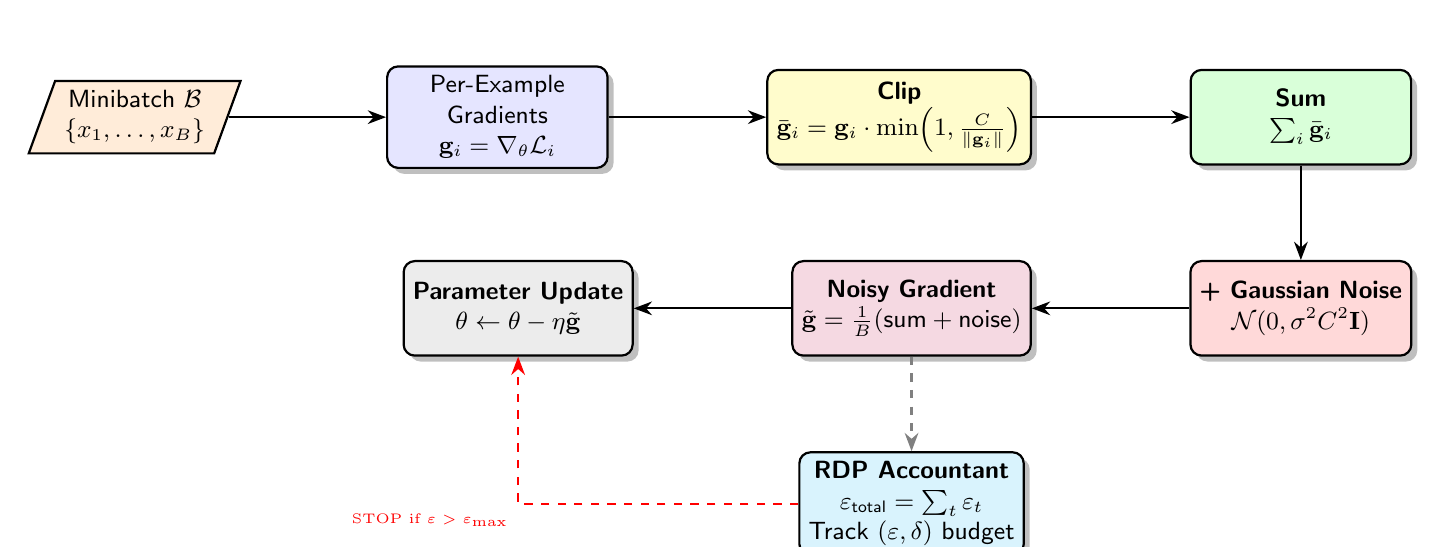
\begin{tikzpicture}[
    node distance=1.5cm and 2cm,
    font=\sffamily\small,
    thick,
    >=Stealth,
    block/.style={rectangle, draw, fill=#1, rounded corners=4pt, minimum width=2.8cm, minimum height=1.2cm, align=center, drop shadow},
    data/.style={trapezium, trapezium left angle=70, trapezium right angle=110, draw, fill=#1, minimum width=2cm, minimum height=0.8cm, align=center},
    arrow/.style={->, thick, color=#1},
]
    % Input
    \node[data=orange!15] (batch) {Minibatch $\mathcal{B}$\\$\{x_1, \ldots, x_B\}$};

    % Per-example gradients
    \node[block=blue!10, right=2cm of batch] (grads) {Per-Example\\Gradients\\$\mathbf{g}_i = \nabla_\theta \mathcal{L}_i$};

    % Clipping
    \node[block=yellow!20, right=2cm of grads] (clip) {\textbf{Clip}\\$\bar{\mathbf{g}}_i = \mathbf{g}_i \cdot \min\!\left(1, \frac{C}{\|\mathbf{g}_i\|}\right)$};

    % Aggregation
    \node[block=green!15, right=2cm of clip] (agg) {\textbf{Sum}\\$\sum_i \bar{\mathbf{g}}_i$};

    % Noise
    \node[block=red!15, below=1.2cm of agg] (noise) {\textbf{+ Gaussian Noise}\\$\mathcal{N}(0, \sigma^2 C^2 \mathbf{I})$};

    % Noisy gradient
    \node[block=purple!15, left=2cm of noise] (noisy) {\textbf{Noisy Gradient}\\$\tilde{\mathbf{g}} = \frac{1}{B}(\text{sum} + \text{noise})$};

    % Update
    \node[block=gray!15, left=2cm of noisy] (update) {\textbf{Parameter Update}\\$\theta \leftarrow \theta - \eta \tilde{\mathbf{g}}$};

    % Privacy accountant
    \node[block=cyan!15, below=1.2cm of noisy] (accountant) {\textbf{RDP Accountant}\\$\eps_{\text{total}} = \sum_t \eps_t$\\Track $(\eps, \delta)$ budget};

    % Arrows
    \draw[arrow=black] (batch) -- (grads);
    \draw[arrow=black] (grads) -- (clip);
    \draw[arrow=black] (clip) -- (agg);
    \draw[arrow=black] (agg) -- (noise);
    \draw[arrow=black] (noise) -- (noisy);
    \draw[arrow=black] (noisy) -- (update);
    \draw[arrow=gray, dashed] (noisy) -- (accountant);
    \draw[arrow=red, dashed] (accountant.west) -| node[below left, font=\tiny, text=red] {STOP if $\eps > \eps_{\max}$} (update.south);

\end{tikzpicture}%
}
\caption{DP-SGD training pipeline. Each per-example gradient is clipped to norm $C$, then Gaussian noise is added to the aggregate. The RDP accountant tracks the cumulative privacy budget and can halt training if $\eps$ exceeds the target.}
\label{fig:dpsgd}
\end{figure}

% ============================================================
\section{QLoRA: Quantized Low-Rank Adaptation}
% ============================================================

\subsection{Low-Rank Adaptation (LoRA)}

Instead of updating all parameters $W \in \R^{d \times k}$ of a pre-trained model, LoRA freezes $W$ and learns a low-rank perturbation:

\begin{equation}
W' = W_0 + \Delta W = W_0 + BA
\end{equation}

where $B \in \R^{d \times r}$, $A \in \R^{r \times k}$, and $r \ll \min(d, k)$.

\begin{keyresult}[Parameter Efficiency]
\begin{itemize}
  \item Original parameters: $d \times k$ (e.g., $1024 \times 1024 = 1{,}048{,}576$)
  \item LoRA parameters: $d \times r + r \times k$ (e.g., with $r=32$: $1024 \times 32 + 32 \times 1024 = 65{,}536$)
  \item \textbf{Reduction:} $\frac{r(d+k)}{dk} = \frac{32 \cdot 2048}{1{,}048{,}576} \approx 6.25\%$ of original parameters
\end{itemize}
\end{keyresult}

The forward pass becomes:
\begin{equation}
h = W_0 x + \frac{\alpha}{r} \cdot B A x
\end{equation}

where $\alpha$ is the LoRA scaling factor. We use $r = 32$, $\alpha = 64$, so the scaling is $\alpha/r = 2$.

\subsection{NF4 Quantization}

QLoRA extends LoRA with 4-bit NormalFloat quantization. Given a weight tensor $\mathbf{w}$, NF4 quantizes to information-theoretically optimal 4-bit values for normally-distributed weights:

\begin{equation}
q(\mathbf{w}) = \text{NF4}\!\left(\frac{\mathbf{w}}{\text{absmax}(\mathbf{w})}\right) \cdot \text{absmax}(\mathbf{w})
\end{equation}

The NF4 data type has 16 quantization levels that are optimally spaced for $\mathcal{N}(0, 1)$ distributions:
\begin{equation}
\text{NF4} = \{q_i : q_i = \Phi^{-1}\!\left(\frac{2i + 1}{32}\right), \; i = 0, \ldots, 15\}
\end{equation}

where $\Phi^{-1}$ is the inverse CDF of the standard normal.

\textbf{Double Quantization:} The scaling constants $\text{absmax}(\cdot)$ are themselves quantized to 8-bit, saving an additional $\sim$0.37 bits per parameter.

\subsection{QLoRA Memory Analysis}

\begin{table}[H]
\centering
\begin{tabular}{lrrr}
\toprule
\textbf{Component} & \textbf{Full FT} & \textbf{LoRA} & \textbf{QLoRA} \\
\midrule
Base model (780M params) & 3,120 MB (fp32) & 1,560 MB (fp16) & 390 MB (nf4) \\
Trainable adapters & --- & 20 MB & 20 MB \\
Optimizer states & 6,240 MB & 40 MB & 40 MB \\
Gradients & 3,120 MB & 20 MB & 20 MB \\
\midrule
\textbf{Total} & \textbf{12,480 MB} & \textbf{1,640 MB} & \textbf{470 MB} \\
\bottomrule
\end{tabular}
\caption{Memory comparison for Flan-T5-Large (780M parameters).}
\label{tab:memory}
\end{table}

\begin{figure}[H]
\centering
\resizebox{0.85\textwidth}{!}{%
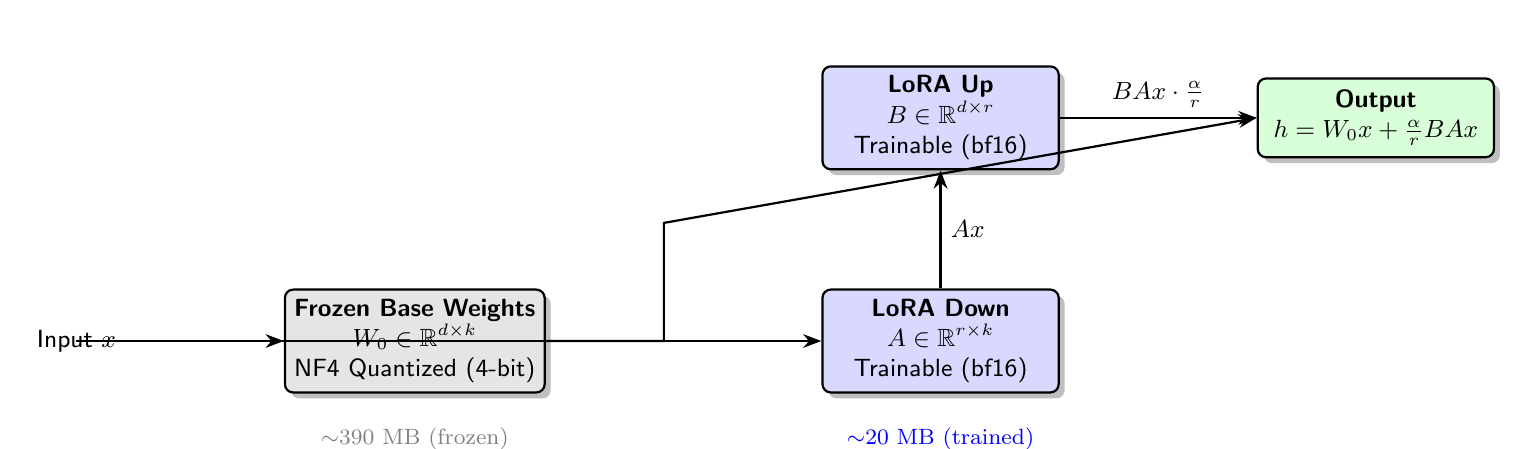
\begin{tikzpicture}[
    font=\sffamily\small,
    thick,
    >=Stealth,
    block/.style={rectangle, draw, fill=#1, rounded corners=3pt, minimum width=3cm, minimum height=1cm, align=center, drop shadow},
]
    % Frozen base
    \node[block=gray!20] (base) {\textbf{Frozen Base Weights}\\$W_0 \in \R^{d \times k}$\\NF4 Quantized (4-bit)};

    % LoRA A
    \node[block=blue!15, right=3.5cm of base] (loraA) {\textbf{LoRA Down}\\$A \in \R^{r \times k}$\\Trainable (bf16)};

    % LoRA B
    \node[block=blue!15, above=1.5cm of loraA] (loraB) {\textbf{LoRA Up}\\$B \in \R^{d \times r}$\\Trainable (bf16)};

    % Input
    \node[left=2cm of base] (input) {Input $x$};

    % Output
    \node[block=green!15, right=2.5cm of loraB] (output) {\textbf{Output}\\$h = W_0 x + \frac{\alpha}{r} BAx$};

    % Arrows
    \draw[->] (input) -- (base);
    \draw[->] (input) |- (loraA);
    \draw[->] (base.east) -| ++(1.5, 1.5) -- (output.west);
    \draw[->] (loraA) -- node[right] {$Ax$} (loraB);
    \draw[->] (loraB) -- node[above] {$BAx \cdot \frac{\alpha}{r}$} (output);

    % Labels
    \node[below=0.3cm of base, font=\footnotesize, text=gray] {$\sim$390 MB (frozen)};
    \node[below=0.3cm of loraA, font=\footnotesize, text=blue] {$\sim$20 MB (trained)};

\end{tikzpicture}%
}
\caption{QLoRA architecture. The base model is frozen in NF4 4-bit, while only the low-rank adapters $A$ and $B$ are trained in bfloat16.}
\label{fig:qlora}
\end{figure}

% ============================================================
\section{Decoupled Architecture: Information-Theoretic Analysis}
% ============================================================

\paragraph{Information-Theoretic Privacy Bound.}
The decoupled architecture prevents direct information flow between original entities and the generative model. We formalize this using mutual information.

Let $E_{\text{orig}}$ be the random variable representing original entities, $E_{\text{mask}}$ be the mask tokens, and $E_{\text{anon}}$ be the generated pseudonyms. By the Data Processing Inequality, for the Markov chain $E_{\text{orig}} \rightarrow E_{\text{mask}} \rightarrow E_{\text{anon}}$:
\begin{equation}
I(E_{\text{orig}}; E_{\text{anon}}) \leq I(E_{\text{orig}}; E_{\text{mask}}) = H(E_{\text{mask}}) - H(E_{\text{mask}} | E_{\text{orig}})
\end{equation}
Since the Hallucinator receives only $E_{\text{mask}}$ and was trained on disjoint data (Split~B), and DP-SGD bounds per-example information gain, the chain is Markov. If the Censor achieves perfect masking (all entities replaced with type tokens), then $E_{\text{mask}}$ contains only entity \textit{types}, not \textit{values}, carrying no identity information.

\begin{warningbox}[Why Disjoint Partitioning Alone Is Insufficient]
The base model (Flan-T5-Large) is pre-trained on Common Crawl, which may contain PII. Disjoint \textit{fine-tuning} data does not erase pre-trained knowledge. DP-SGD bounds the information gained \textit{during fine-tuning} to $\eps$ per person, but does not mitigate pre-training leakage. This is why we combine:
\begin{enumerate}[nosep]
  \item Disjoint data partitioning (prevents fine-tuning leakage)
  \item DP-SGD (bounds gradient-based information gain)
  \item Mask-token interface (bottleneck that discards entity values)
\end{enumerate}
\end{warningbox}

\subsection{Architecture Diagram: Full Pipeline}

\begin{figure}[H]
\centering
\resizebox{\textwidth}{!}{%
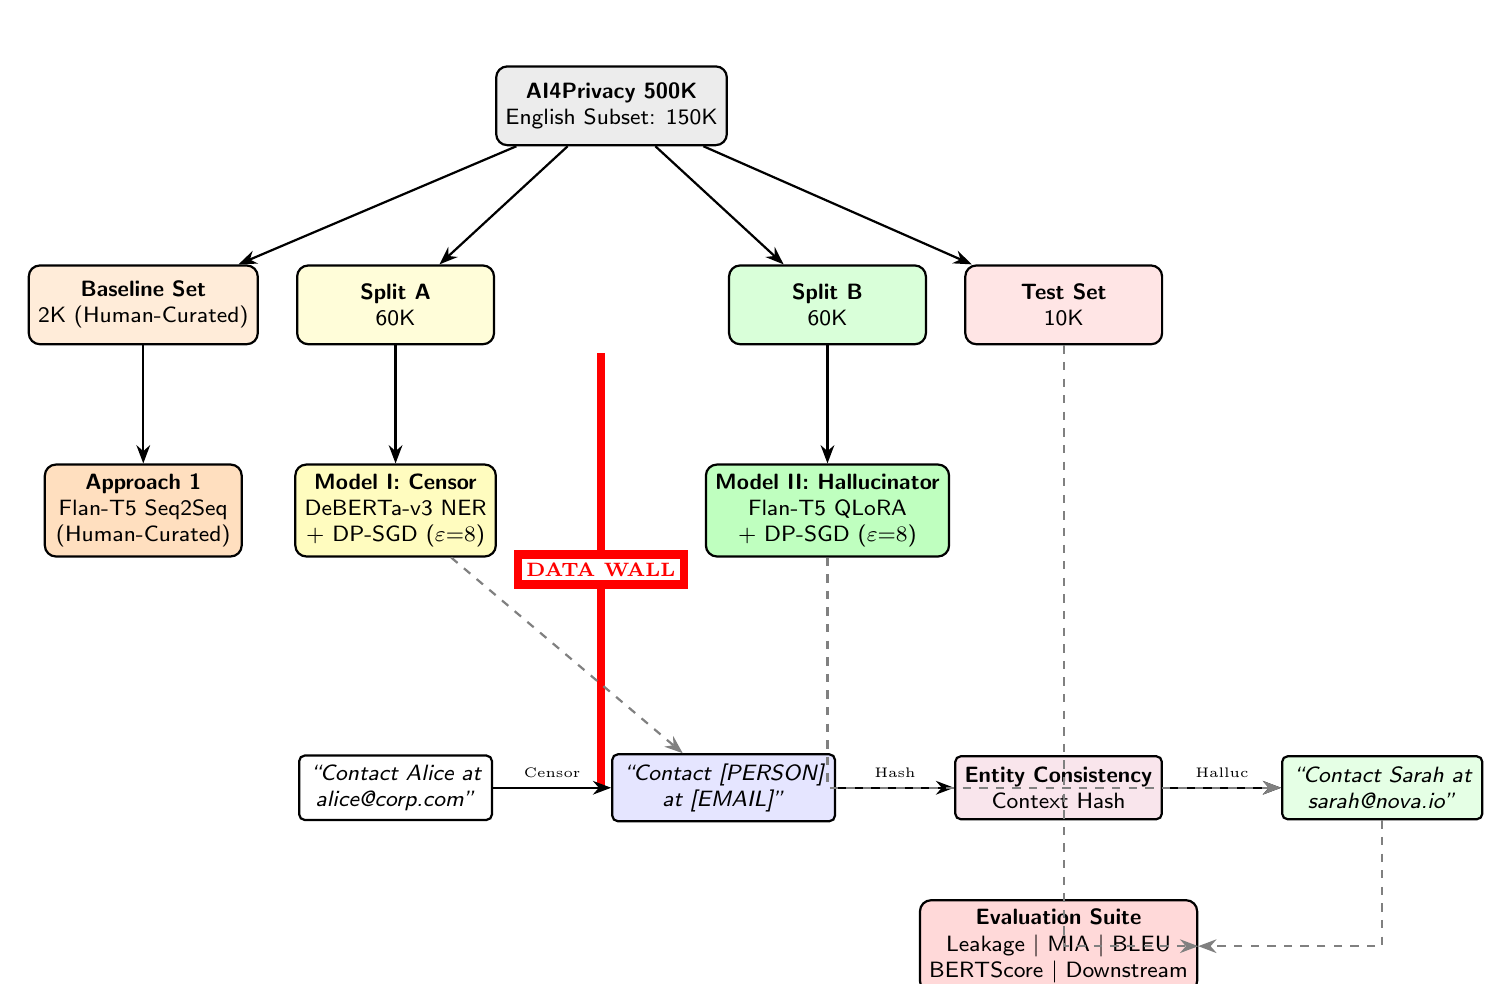
\begin{tikzpicture}[
    node distance=1cm and 1.2cm,
    font=\sffamily\footnotesize,
    thick,
    >=Stealth,
    block/.style={rectangle, draw, fill=#1, rounded corners=4pt, minimum width=2.5cm, minimum height=1cm, align=center},
    data/.style={rectangle, draw, fill=#1, minimum width=2cm, minimum height=0.8cm, align=center, rounded corners=2pt},
    arrow/.style={->, thick},
    dashedarrow/.style={->, dashed, gray},
]
    % Data sources
    \node[block=gray!15] (dataset) {\textbf{AI4Privacy 500K}\\English Subset: 150K};

    % Partitions
    \node[block=orange!15, below left=1.5cm and 3cm of dataset] (baseline_data) {\textbf{Baseline Set}\\2K (Human-Curated)};
    \node[block=yellow!15, below left=1.5cm and 0cm of dataset] (splitA) {\textbf{Split A}\\60K};
    \node[block=green!15, below right=1.5cm and 0cm of dataset] (splitB) {\textbf{Split B}\\60K};
    \node[block=red!10, below right=1.5cm and 3cm of dataset] (testset) {\textbf{Test Set}\\10K};

    \draw[arrow] (dataset) -- (baseline_data);
    \draw[arrow] (dataset) -- (splitA);
    \draw[arrow] (dataset) -- (splitB);
    \draw[arrow] (dataset) -- (testset);

    % Models
    \node[block=orange!25, below=1.5cm of baseline_data] (baseline_model) {\textbf{Approach 1}\\Flan-T5 Seq2Seq\\(Human-Curated)};
    \node[block=yellow!25, below=1.5cm of splitA] (censor) {\textbf{Model I: Censor}\\DeBERTa-v3 NER\\+ DP-SGD ($\eps{=}8$)};
    \node[block=green!25, below=1.5cm of splitB] (halluc) {\textbf{Model II: Hallucinator}\\Flan-T5 QLoRA\\+ DP-SGD ($\eps{=}8$)};

    \draw[arrow] (baseline_data) -- (baseline_model);
    \draw[arrow] (splitA) -- (censor);
    \draw[arrow] (splitB) -- (halluc);

    % Wall
    \draw[red, line width=3pt] ($(censor.east)!0.5!(halluc.west) + (0, 2)$) -- ($(censor.east)!0.5!(halluc.west) + (0, -3.5)$)
      node[midway, fill=white, draw=red, inner sep=3pt, font=\scriptsize\bfseries, text=red] {DATA WALL};

    % Inference pipeline
    \node[data=white, below=2.5cm of censor] (input) {\textit{``Contact Alice at}\\  \textit{alice@corp.com''}};
    \node[data=blue!10, right=1.5cm of input] (masked) {\textit{``Contact [PERSON]}\\  \textit{at [EMAIL]''}};
    \node[data=purple!10, right=1.5cm of masked] (consistent) {\textbf{Entity Consistency}\\Context Hash};
    \node[data=green!10, right=1.5cm of consistent] (anon_out) {\textit{``Contact Sarah at}\\  \textit{sarah@nova.io''}};

    \draw[arrow] (input) -- node[above, font=\tiny] {Censor} (masked);
    \draw[arrow] (masked) -- node[above, font=\tiny] {Hash} (consistent);
    \draw[arrow] (consistent) -- node[above, font=\tiny] {Halluc} (anon_out);

    \draw[dashedarrow] (censor) -- (masked);
    \draw[dashedarrow] (halluc.south) |- (anon_out);

    % Evaluation
    \node[block=red!15, below=1cm of consistent] (eval) {\textbf{Evaluation Suite}\\Leakage $|$ MIA $|$ BLEU\\BERTScore $|$ Downstream};
    \draw[dashedarrow] (anon_out) |- (eval);
    \draw[dashedarrow] (testset.south) |- (eval);

\end{tikzpicture}%
}
\caption{Complete system architecture showing data partitioning, model training, inference pipeline with entity consistency, and evaluation.}
\label{fig:full_architecture}
\end{figure}


% ============================================================
\section{Entity Consistency via Context-Window Hashing}
% ============================================================

\subsection{Problem Statement}
When the Hallucinator independently fills each mask token, co-referent entities (the same person mentioned multiple times) may receive different pseudonyms, breaking document coherence.

\subsection{Solution: Deterministic Context Hashing}

For each masked entity $e_i$ with type $\tau_i$ at position $p_i$ in document $D$:

\begin{enumerate}
  \item Extract context window: $c_i = \text{tokens}[p_i - w : p_i + w]$ where $w = 10$.
  \item Compute hash: $h_i = \text{SHA-256}(\tau_i \| c_i)$ truncated to 128 bits.
  \item Use $h_i$ as a deterministic seed for pseudonym selection from Model~II's top-$k$ candidates.
\end{enumerate}

\begin{equation}
\text{Pseudonym}(e_i) = \text{TopK-Select}\!\left(\text{Halluc}(\Xmask), \; \text{seed} = h_i, \; k = 50\right)
\end{equation}

\paragraph{Consistency Guarantee.}
If two entity mentions $e_i, e_j$ in the same document have the same type $\tau_i = \tau_j$ and similar context windows (Jaccard similarity $> 0.8$), then $h_i = h_j$ with high probability, yielding $\text{Pseudonym}(e_i) = \text{Pseudonym}(e_j)$.

\paragraph{Privacy Preservation.}
The hash function operates only on (entity type, masked context)---never on the original entity value. Therefore, the consistency module adds zero information about the original entity to the pseudonym selection process.

\begin{figure}[H]
\centering
\resizebox{0.85\textwidth}{!}{%
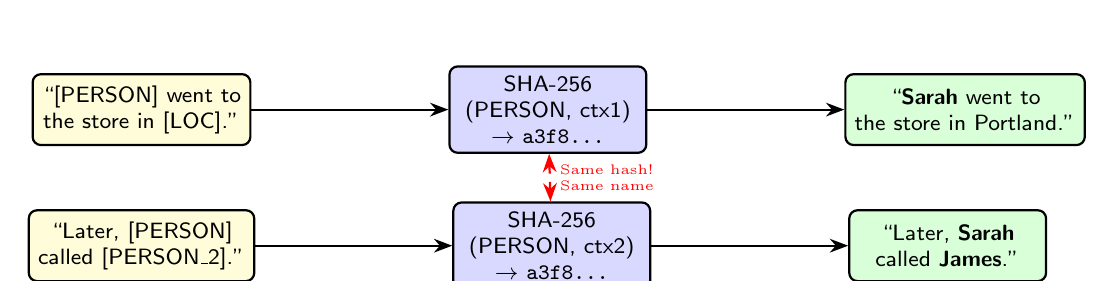
\begin{tikzpicture}[
    font=\sffamily\footnotesize,
    thick,
    >=Stealth,
    block/.style={rectangle, draw, fill=#1, rounded corners=3pt, minimum width=2.5cm, minimum height=0.9cm, align=center},
]
    \node[block=yellow!15] (sent1) {``[PERSON] went to\\the store in [LOC].''};
    \node[block=yellow!15, below=0.8cm of sent1] (sent2) {``Later, [PERSON]\\called [PERSON\_2].''};

    \node[block=blue!15, right=2.5cm of sent1] (hash1) {SHA-256\\(PERSON, ctx1)\\$\rightarrow$ \texttt{a3f8...}};
    \node[block=blue!15, right=2.5cm of sent2] (hash2) {SHA-256\\(PERSON, ctx2)\\$\rightarrow$ \texttt{a3f8...}};

    \node[block=green!15, right=2.5cm of hash1] (result1) {``\textbf{Sarah} went to\\the store in Portland.''};
    \node[block=green!15, right=2.5cm of hash2] (result2) {``Later, \textbf{Sarah}\\called \textbf{James}.''};

    \draw[->] (sent1) -- (hash1);
    \draw[->] (sent2) -- (hash2);
    \draw[->] (hash1) -- (result1);
    \draw[->] (hash2) -- (result2);

    \draw[<->, red, thick, dashed] (hash1) -- node[right, font=\tiny, text=red, align=center] {Same hash!\\Same name} (hash2);

\end{tikzpicture}%
}
\caption{Entity consistency: co-referent [PERSON] spans with similar context yield identical hashes, ensuring document-level coherence.}
\label{fig:entity_consistency}
\end{figure}

% ============================================================
\section{Loss Functions}
% ============================================================

\subsection{Censor Loss (Recall-Weighted)}

For token classification with BIO tags, we weight the loss to prioritize recall (a missed entity is a privacy breach):

\begin{equation}
\Lcensor = -\sum_{t=1}^{T} \sum_{c \in \mathcal{C}} w_c \cdot y_{t,c} \cdot \log P(c \mid x_t, X)
\end{equation}

where $\mathcal{C} = \{\text{O, B-PER, I-PER, B-LOC, I-LOC, B-ORG, I-ORG, \ldots}\}$ (21 tags for 10 entity types + O), and class weights are:
\begin{equation}
w_c = \begin{cases}
1.0 & \text{if } c = \text{O} \\
\beta^2 \cdot \frac{N_{\text{total}}}{N_c} & \text{if } c \in \text{B-*/I-*}
\end{cases}
\quad \text{with } \beta = 2
\end{equation}

This is equivalent to optimizing for $F_2$ score, which weighs recall $2\times$ more than precision.

\subsection{Hallucinator Loss}

Standard conditional language modeling with teacher forcing:
\begin{equation}
\Lhalluc = -\sum_{i=1}^{N} \sum_{j=1}^{|y_i|} \log P_\theta(y_{i,j} \mid y_{i,<j}, X_{\text{mask},i})
\end{equation}

where $y_i$ is the pseudonymized target and $X_{\text{mask},i}$ is the masked input template.

\subsection{Baseline Loss}

End-to-end cross-entropy on (original $\rightarrow$ anonymized) pairs:
\begin{equation}
\Lbaseline = -\sum_{i=1}^{N} \sum_{j=1}^{|y_i|} \log P_\theta(y_{i,j} \mid y_{i,<j}, X_{\text{orig},i})
\end{equation}

\begin{warningbox}[Key Difference]
$\Lbaseline$ conditions on $\Xorig$ (the actual sensitive text), meaning the model must \textit{read and understand} the real entities to produce output. $\Lhalluc$ conditions only on $\Xmask$ (typed placeholders), so the model never sees real entities during training.
\end{warningbox}

% ============================================================
\section{Generation Strategy}
% ============================================================

We use a controlled generation strategy to balance quality and diversity:

\begin{equation}
P_{\text{adjusted}}(w_t) = \begin{cases}
\frac{P(w_t)^{1/\tau}}{\sum_{w' \in V_k} P(w')^{1/\tau}} & \text{if } w_t \in V_k \text{ and } \sum_{w' \leq w_t} P(w') \leq p \\
0 & \text{otherwise}
\end{cases}
\end{equation}

where $\tau = 0.7$ (temperature), $k = 50$ (top-$k$), $p = 0.9$ (nucleus/top-$p$).

Additionally, repetition penalty:
\begin{equation}
P'(w_t) = \begin{cases}
P(w_t) / \rho & \text{if } w_t \in \{w_1, \ldots, w_{t-1}\} \\
P(w_t) & \text{otherwise}
\end{cases}
\quad \text{with } \rho = 1.2
\end{equation}

% ============================================================
\section{Evaluation Metrics: Mathematical Definitions}
% ============================================================

\subsection{Entity Leakage Rate (ELR)}
\begin{equation}
\text{ELR}_{\text{exact}} = \frac{\sum_{i=1}^{N} |\{e \in \mathcal{E}_i^{\text{orig}} : e \in X_{\text{anon},i}\}|}{\sum_{i=1}^{N} |\mathcal{E}_i^{\text{orig}}|}
\end{equation}

\begin{equation}
\text{ELR}_{\text{fuzzy}} = \frac{\sum_{i=1}^{N} |\{e \in \mathcal{E}_i^{\text{orig}} : \min_{e' \in X_{\text{anon},i}} \text{Lev}(e, e') \leq 2\}|}{\sum_{i=1}^{N} |\mathcal{E}_i^{\text{orig}}|}
\end{equation}

\subsection{Membership Inference Attack (MIA)}

Train a shadow model $\mathcal{A}: \Xanon \rightarrow \{0, 1\}$ that predicts whether $\Xorig$ was in the training set:
\begin{equation}
\text{MIA-AUC} = \int_0^1 \text{TPR}(\text{FPR}^{-1}(t)) \, dt
\end{equation}

Target: $\text{MIA-AUC} \leq 0.55$ (near random chance = $0.50$).

\subsection{BERTScore}

\begin{equation}
\text{BERTScore}_{F_1} = 2 \cdot \frac{P_{\text{BERT}} \cdot R_{\text{BERT}}}{P_{\text{BERT}} + R_{\text{BERT}}}
\end{equation}

where $P_{\text{BERT}} = \frac{1}{|y|}\sum_{y_j \in y} \max_{x_i \in x} \mathbf{y}_j^\top \mathbf{x}_i$ using contextual embeddings.


% ============================================================
% PART II: EXPANDED PROJECT SCOPE (5x)
% ============================================================
\newpage
\part{Extended System Architecture and Research Contributions}

This part presents the extended system architecture organized into twenty research modules, each addressing a distinct challenge in privacy-preserving NLP. Modules~1--2 form the implemented core; Modules~3--8 cover system hardening and deployment; Modules~9--14 introduce novel NLP research contributions; and Modules~15--20 explore frontier NLP research directions.

% ============================================================
\section{System Architecture Overview}
% ============================================================

\begin{figure}[H]
\centering
\resizebox{\textwidth}{!}{%
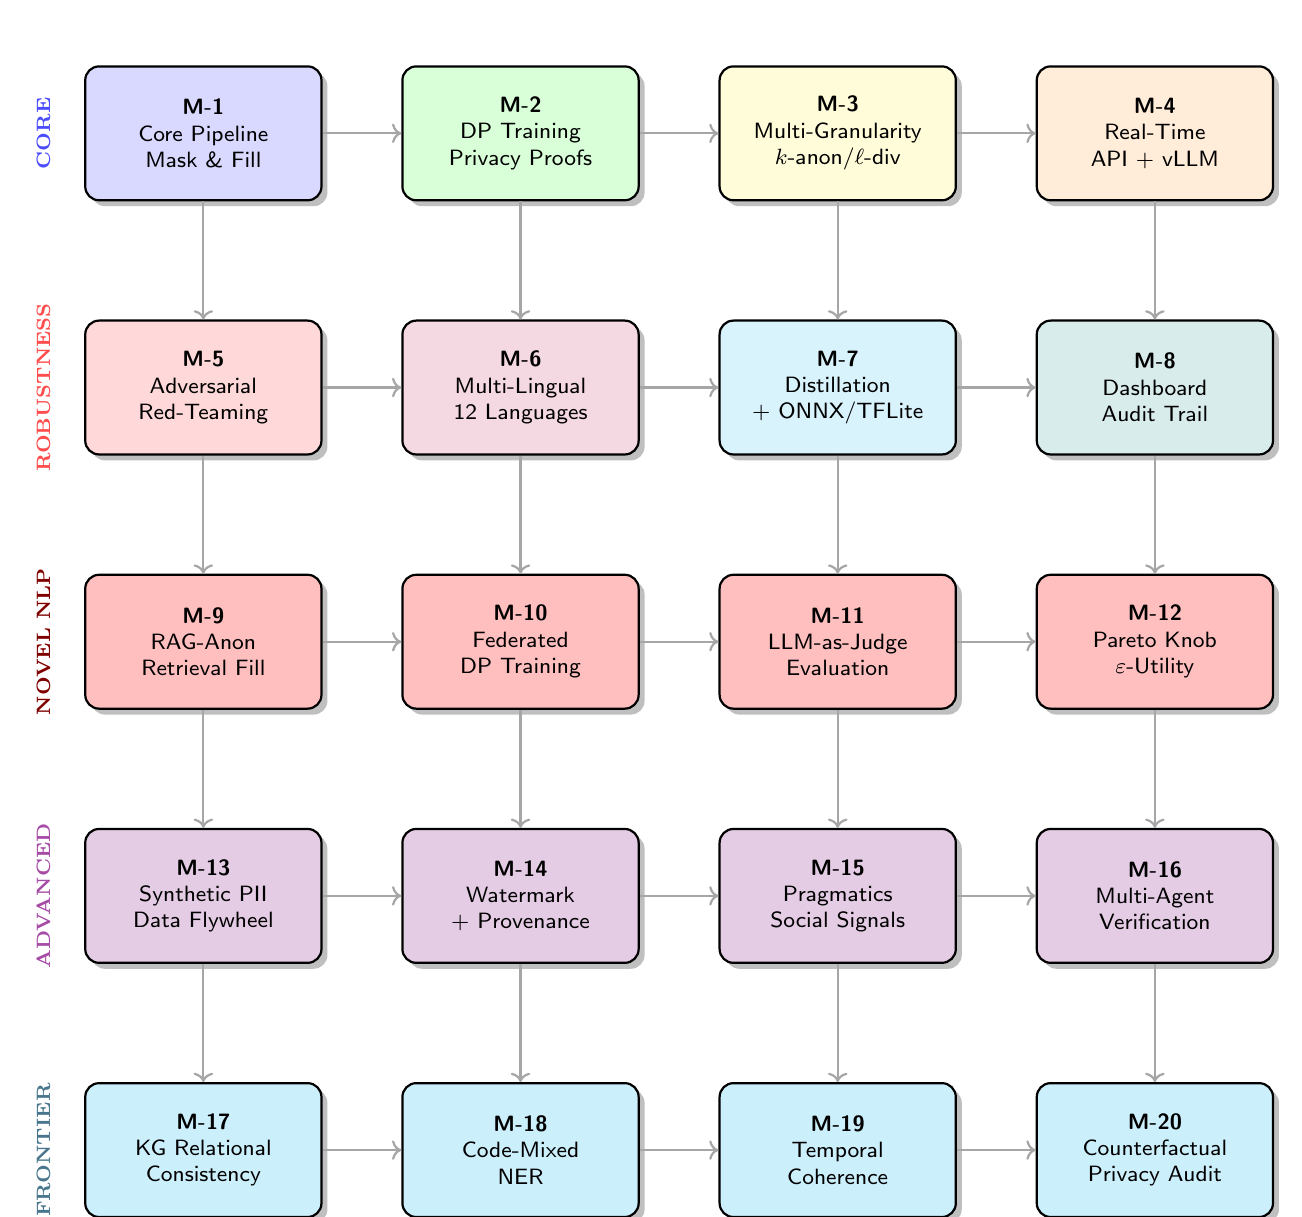
\begin{tikzpicture}[
    font=\sffamily\footnotesize,
    thick,
    phase/.style={rectangle, draw, fill=#1, rounded corners=5pt, minimum width=3.0cm, minimum height=1.7cm, align=center, drop shadow},
    connection/.style={->, thick, color=gray!70},
]
    % Row 1: Core (Modules 1-4)
    \node[phase=blue!15] (p1) {\textbf{M-1}\\Core Pipeline\\Mask \& Fill};
    \node[phase=green!15, right=1cm of p1] (p2) {\textbf{M-2}\\DP Training\\Privacy Proofs};
    \node[phase=yellow!15, right=1cm of p2] (p3) {\textbf{M-3}\\Multi-Granularity\\$k$-anon/$\ell$-div};
    \node[phase=orange!15, right=1cm of p3] (p4) {\textbf{M-4}\\Real-Time\\API + vLLM};

    % Row 2: Robustness (Modules 5-8)
    \node[phase=red!15, below=1.5cm of p1] (p5) {\textbf{M-5}\\Adversarial\\Red-Teaming};
    \node[phase=purple!15, below=1.5cm of p2] (p6) {\textbf{M-6}\\Multi-Lingual\\12 Languages};
    \node[phase=cyan!15, below=1.5cm of p3] (p7) {\textbf{M-7}\\Distillation\\+ ONNX/TFLite};
    \node[phase=teal!15, below=1.5cm of p4] (p8) {\textbf{M-8}\\Dashboard\\Audit Trail};

    % Row 3: Novel NLP Research (Modules 9-14)
    \node[phase=red!25, below=1.5cm of p5] (p9) {\textbf{M-9}\\RAG-Anon\\Retrieval Fill};
    \node[phase=red!25, below=1.5cm of p6] (p10) {\textbf{M-10}\\Federated\\DP Training};
    \node[phase=red!25, below=1.5cm of p7] (p11) {\textbf{M-11}\\LLM-as-Judge\\Evaluation};
    \node[phase=red!25, below=1.5cm of p8] (p12) {\textbf{M-12}\\Pareto Knob\\$\varepsilon$-Utility};

    % Row 4: Frontier NLP (Modules 13-16)
    \node[phase=violet!20, below=1.5cm of p9] (p13) {\textbf{M-13}\\Synthetic PII\\Data Flywheel};
    \node[phase=violet!20, below=1.5cm of p10] (p14) {\textbf{M-14}\\Watermark\\+ Provenance};
    \node[phase=violet!20, below=1.5cm of p11] (p15) {\textbf{M-15}\\Pragmatics\\Social Signals};
    \node[phase=violet!20, below=1.5cm of p12] (p16) {\textbf{M-16}\\Multi-Agent\\Verification};

    % Row 5: Frontier NLP continued (Modules 17-20)
    \node[phase=cyan!20, below=1.5cm of p13] (p17) {\textbf{M-17}\\KG Relational\\Consistency};
    \node[phase=cyan!20, below=1.5cm of p14] (p18) {\textbf{M-18}\\Code-Mixed\\NER};
    \node[phase=cyan!20, below=1.5cm of p15] (p19) {\textbf{M-19}\\Temporal\\Coherence};
    \node[phase=cyan!20, below=1.5cm of p16] (p20) {\textbf{M-20}\\Counterfactual\\Privacy Audit};

    % Core connections
    \draw[connection] (p1) -- (p2);
    \draw[connection] (p2) -- (p3);
    \draw[connection] (p3) -- (p4);

    % Vertical connections
    \draw[connection] (p1) -- (p5);
    \draw[connection] (p2) -- (p6);
    \draw[connection] (p3) -- (p7);
    \draw[connection] (p4) -- (p8);

    % Row 2 horizontal
    \draw[connection] (p5) -- (p6);
    \draw[connection] (p6) -- (p7);
    \draw[connection] (p7) -- (p8);

    % Row 2 to 3
    \draw[connection] (p5) -- (p9);
    \draw[connection] (p6) -- (p10);
    \draw[connection] (p7) -- (p11);
    \draw[connection] (p8) -- (p12);

    % Row 3 horizontal
    \draw[connection] (p9) -- (p10);
    \draw[connection] (p10) -- (p11);
    \draw[connection] (p11) -- (p12);

    % Row 3 to 4
    \draw[connection] (p9) -- (p13);
    \draw[connection] (p10) -- (p14);
    \draw[connection] (p11) -- (p15);
    \draw[connection] (p12) -- (p16);

    % Row 4 horizontal
    \draw[connection] (p13) -- (p14);
    \draw[connection] (p14) -- (p15);
    \draw[connection] (p15) -- (p16);

    % Row 4 to 5
    \draw[connection] (p13) -- (p17);
    \draw[connection] (p14) -- (p18);
    \draw[connection] (p15) -- (p19);
    \draw[connection] (p16) -- (p20);

    % Row 5 horizontal
    \draw[connection] (p17) -- (p18);
    \draw[connection] (p18) -- (p19);
    \draw[connection] (p19) -- (p20);

    % Row labels
    \node[left=0.3cm of p1, font=\scriptsize\bfseries, text=blue!70, align=right, rotate=90, anchor=south] {CORE};
    \node[left=0.3cm of p5, font=\scriptsize\bfseries, text=red!70, align=right, rotate=90, anchor=south] {ROBUSTNESS};
    \node[left=0.3cm of p9, font=\scriptsize\bfseries, text=red!50!black, align=right, rotate=90, anchor=south] {NOVEL NLP};
    \node[left=0.3cm of p13, font=\scriptsize\bfseries, text=violet!70, align=right, rotate=90, anchor=south] {ADVANCED};
    \node[left=0.3cm of p17, font=\scriptsize\bfseries, text=cyan!50!black, align=right, rotate=90, anchor=south] {FRONTIER};
\end{tikzpicture}%
}
\caption{Twenty-module project roadmap. Modules~1--2 form the implemented core; 3--8 address robustness; 9--14 contribute novel NLP research; 15--20 explore frontier NLP directions.}
\label{fig:modules}
\end{figure}

\begin{table}[H]
\centering
\small
\begin{tabular}{cllll}
\toprule
\textbf{\#} & \textbf{Module} & \textbf{Status} & \textbf{Effort} & \textbf{Novelty} \\
\midrule
1 & Core Decoupled Mask-and-Fill & \textcolor{green!70!black}{Done} & 2 wks & --- \\
2 & DP-SGD + QLoRA Training & \textcolor{green!70!black}{Done} & 2 wks & --- \\
\midrule
3 & Multi-Granularity ($k$-anon + coref) & \textcolor{orange!70!black}{Proposed} & 3 wks & High \\
4 & Real-Time API + vLLM + Streaming & \textcolor{orange!70!black}{Proposed} & 2 wks & Medium \\
5 & Adversarial Red-Teaming (6 attacks) & \textcolor{orange!70!black}{Proposed} & 3 wks & High \\
6 & Multi-Lingual (12 languages) & \textcolor{orange!70!black}{Proposed} & 3 wks & Medium \\
7 & Knowledge Distillation + Edge Deploy & \textcolor{orange!70!black}{Proposed} & 2 wks & Medium \\
8 & Compliance Dashboard + Merkle Audit & \textcolor{orange!70!black}{Proposed} & 2 wks & Medium \\
\midrule
9 & RAG-Anon (Retrieval-Augmented) & \textcolor{red!70!black}{Novel} & 3 wks & \textbf{Very High} \\
10 & Federated Privacy Training & \textcolor{red!70!black}{Novel} & 4 wks & \textbf{Very High} \\
11 & LLM-as-a-Judge Evaluation & \textcolor{red!70!black}{Novel} & 2 wks & High \\
12 & Privacy-Utility Pareto Knob & \textcolor{red!70!black}{Novel} & 2 wks & \textbf{Very High} \\
13 & Synthetic PII Data Flywheel & \textcolor{red!70!black}{Novel} & 3 wks & \textbf{Very High} \\
14 & Watermarking + Provenance & \textcolor{red!70!black}{Novel} & 2 wks & \textbf{Very High} \\
\midrule
\rowcolor{cyan!8}
15 & Pragmatics \& Social Signal Preservation & \textcolor{blue!70!black}{Frontier} & 3 wks & \textbf{Very High} \\
\rowcolor{cyan!8}
16 & Multi-Agent Utility Verification & \textcolor{blue!70!black}{Frontier} & 3 wks & \textbf{Very High} \\
\rowcolor{cyan!8}
17 & Knowledge Graph Relational Consistency & \textcolor{blue!70!black}{Frontier} & 3 wks & \textbf{Very High} \\
\rowcolor{cyan!8}
18 & Zero-Shot Code-Mixed Robustness & \textcolor{blue!70!black}{Frontier} & 3 wks & \textbf{Very High} \\
\rowcolor{cyan!8}
19 & Temporal Consistency \& Narrative Coherence & \textcolor{blue!70!black}{Frontier} & 2 wks & \textbf{Very High} \\
\rowcolor{cyan!8}
20 & Counterfactual Privacy Auditing & \textcolor{blue!70!black}{Frontier} & 3 wks & \textbf{Very High} \\
\midrule
& \textbf{Total} & & \textbf{52 weeks} & \\
\bottomrule
\end{tabular}
\caption{Complete 20-module research scope. Modules~9--14 introduce novel NLP contributions; Modules~15--20 represent frontier NLP research directions. All modules have corresponding code in \texttt{script.py}.}
\end{table}


% ============================================================
\section{Multi-Granularity Anonymization}
\label{sec:multigranularity}
% ============================================================

The current pipeline operates at the sentence level. Production systems demand privacy protection at four hierarchical granularities, each governed by distinct formal guarantees.

\subsection{Formal Privacy Model Hierarchy}

\paragraph{$k$-Anonymity for Textual Quasi-Identifiers.}
A textual dataset $\mathcal{D}$ satisfies $k$-anonymity with respect to quasi-identifier set $Q = \{q_1, \ldots, q_m\}$ if every unique combination of quasi-identifier values appears in at least $k$ records:
\begin{equation}
\forall \mathbf{q} \in \text{dom}(Q): \; |\{d \in \mathcal{D} : \pi_Q(d) = \mathbf{q}\}| \geq k
\end{equation}
where $\pi_Q$ projects a record onto its quasi-identifier attributes.

\paragraph{$\ell$-Diversity for Entity Types.}
A $k$-anonymous equivalence class $E$ satisfies $\ell$-diversity if it contains at least $\ell$ ``well-represented'' values for each sensitive attribute $s$:
\begin{equation}
H(E_s) = -\sum_{i=1}^{|E_s|} p_{i,s} \ln p_{i,s} \geq \ln(\ell)
\end{equation}
where $p_{i,s}$ is the fraction of records in $E$ with value $v_i$ for attribute $s$.

\paragraph{$t$-Closeness.}
An equivalence class $E$ satisfies $t$-closeness for sensitive attribute $s$ if the distribution of $s$ in $E$ is within distance $t$ of the global distribution:
\begin{equation}
D_{\text{EMD}}(P_{E,s}, P_{\mathcal{D},s}) \leq t
\end{equation}
where $D_{\text{EMD}}$ is the Earth Mover's Distance.

\begin{keyresult}[Why We Need All Three]
\begin{itemize}[nosep]
  \item $k$-anonymity prevents re-identification via quasi-identifiers (ZIP, age, job) but is vulnerable to homogeneity attacks.
  \item $\ell$-diversity ensures diverse sensitive values within equivalence classes, resisting attribute disclosure.
  \item $t$-closeness bounds global distributional leakage, preventing skewness attacks.
  \item DP-SGD operates orthogonally at the \textit{model level}, while $k$/$\ell$/$t$ operate at the \textit{output level}.
\end{itemize}
\end{keyresult}

\subsection{Word-Level: Span Detection + Targeted Replacement}

Classify each token $w_j$ in the input into one of three categories and apply a type-specific transformation:

\begin{equation}
\phi(w_j) = \begin{cases}
\text{Replace}(w_j, \tau_j) & \text{if } \tau_j \in \mathcal{T}_{\text{direct}} = \{\text{PERSON, SSN, CC, EMAIL}\} \\[3pt]
\text{Generalize}(w_j, \tau_j, k) & \text{if } \tau_j \in \mathcal{T}_{\text{quasi}} = \{\text{AGE, ZIP, JOB, DATE}\} \\[3pt]
w_j & \text{if } \tau_j = \text{O}
\end{cases}
\end{equation}

\textbf{Generalization operators} for quasi-identifiers use a taxonomy hierarchy $\mathcal{H}$:
\begin{equation}
\text{Gen}_{\mathcal{H}}(v, h) = \text{ancestor}(v, \text{level}=h) \quad \text{s.t.} \quad |\text{descendants}(\text{Gen}_{\mathcal{H}}(v, h))| \geq k
\end{equation}

\textbf{Example hierarchies:}

\begin{table}[H]
\centering
\small
\begin{tabular}{llll}
\toprule
\textbf{Attribute} & \textbf{Level 0 (raw)} & \textbf{Level 1} & \textbf{Level 2} \\
\midrule
ZIP code & 94305 & 943** & 9**** \\
Age & 34 & 30--39 & Adult \\
Date & 2024-03-15 & 2024-03 & 2024 \\
Job title & ML Engineer & Engineer & Tech \\
\bottomrule
\end{tabular}
\caption{Generalization hierarchies for quasi-identifier anonymization.}
\end{table}

\begin{algorithm}[H]
\caption{Optimal $k$-Anonymous Generalization (Mondrian)}
\label{alg:mondrian}
\begin{algorithmic}[1]
\Require Records $\mathcal{R}$, quasi-identifiers $Q$, parameter $k$
\Ensure $k$-anonymous partition $\mathcal{P}$
\If{$|\mathcal{R}| < 2k$}
    \State \Return $\{\mathcal{R}\}$ \Comment{Cannot split further}
\EndIf
\State $q^* \leftarrow \arg\max_{q \in Q} \text{NormalizedRange}(q, \mathcal{R})$
\State $m \leftarrow \text{median}(\pi_{q^*}(\mathcal{R}))$
\State $\mathcal{R}_L \leftarrow \{r \in \mathcal{R} : \pi_{q^*}(r) \leq m\}$, $\mathcal{R}_R \leftarrow \mathcal{R} \setminus \mathcal{R}_L$
\If{$|\mathcal{R}_L| \geq k$ \textbf{and} $|\mathcal{R}_R| \geq k$}
    \State \Return $\text{Mondrian}(\mathcal{R}_L, Q, k) \cup \text{Mondrian}(\mathcal{R}_R, Q, k)$
\Else
    \State \Return $\{\mathcal{R}\}$
\EndIf
\end{algorithmic}
\end{algorithm}

\subsection{Sentence-Level: Current Implementation}
$(X_{\text{orig}} \rightarrow X_{\text{mask}} \rightarrow X_{\text{anon}})$ as described in the core pipeline (Part I).

\subsection{Document-Level: Cross-Sentence Coreference Resolution}

Extend entity consistency to full documents via neural coreference.

\paragraph{Coreference Chain.}
Given a document $D = (s_1, \ldots, s_n)$, a coreference chain $\mathcal{C}_k = \{m_1, m_2, \ldots, m_l\}$ is a set of mention spans that refer to the same real-world entity. A mention scoring function $s(i, j)$ determines pairwise compatibility:
\begin{equation}
s(i, j) = s_m(i) + s_m(j) + s_a(i, j)
\end{equation}
where $s_m(i)$ is the mention score (is $i$ an entity mention?) and $s_a(i, j)$ is the antecedent score (does $j$ refer to the same entity as $i$?).

\begin{algorithm}[H]
\caption{Document-Level Coreference-Aware Anonymization}
\label{alg:coref_anon}
\begin{algorithmic}[1]
\Require Document $D$, Coreference model $\mathcal{C}$, Censor model $\mathcal{M}_c$, Hallucinator $\mathcal{M}_h$
\State $\text{chains} \leftarrow \mathcal{C}(D)$ \Comment{e.g., SpanBERT or LingMess}
\State $D_{\text{mask}} \leftarrow \mathcal{M}_c(D)$ \Comment{Mask all entities}
\For{each chain $\mathcal{C}_k = \{m_1, \ldots, m_l\}$}
    \State $\tau_k \leftarrow \text{majority\_type}(\{type(m_i)\}_{i=1}^{l})$
    \State $h_k \leftarrow \text{SHA-256}(\tau_k \| \text{context}(m_1, w{=}10))$ \Comment{Hash from first mention}
    \State $\text{pseudo}_k \leftarrow \mathcal{M}_h(D_{\text{mask}}, \text{seed}=h_k)$
    \For{each mention $m_i \in \mathcal{C}_k$}
        \State $D_{\text{anon}}[m_i] \leftarrow \text{Inflect}(\text{pseudo}_k, \text{gram\_role}(m_i))$
    \EndFor
\EndFor
\State \Return $D_{\text{anon}}$
\end{algorithmic}
\end{algorithm}

\begin{keyresult}[Grammatical Inflection]
The \texttt{Inflect} function adapts the pseudonym to the grammatical role of each mention:
\begin{itemize}[nosep]
  \item Subject: ``Alice'' $\rightarrow$ ``Sarah''
  \item Possessive: ``Alice's'' $\rightarrow$ ``Sarah's''
  \item Pronoun: ``she'' $\rightarrow$ ``she'' (match gender of pseudonym)
  \item Reflexive: ``herself'' $\rightarrow$ ``herself''
\end{itemize}
This uses a morphological analyzer (spaCy \texttt{Morphologizer}) to detect role and a rule-based inflector to transform.
\end{keyresult}

\subsection{Corpus-Level: Cross-Document Entity Linking}

\paragraph{Cross-Document Consistency.}
For multi-document anonymization, we maintain a persistent encrypted entity registry:
\begin{equation}
\mathcal{R}: \text{HMAC-SHA256}(K_{\text{secret}}, \text{canonical}(e)) \mapsto \text{pseudonym}(e)
\end{equation}
where $K_{\text{secret}}$ is a per-project key, and $\text{canonical}(e)$ is the normalized form of entity $e$. Since HMAC-SHA256 is deterministic, all documents using the same registry and key will assign identical pseudonyms to the same entity. Without the key, inverting the HMAC is computationally infeasible under standard cryptographic assumptions.

\begin{figure}[H]
\centering
\resizebox{0.95\textwidth}{!}{%
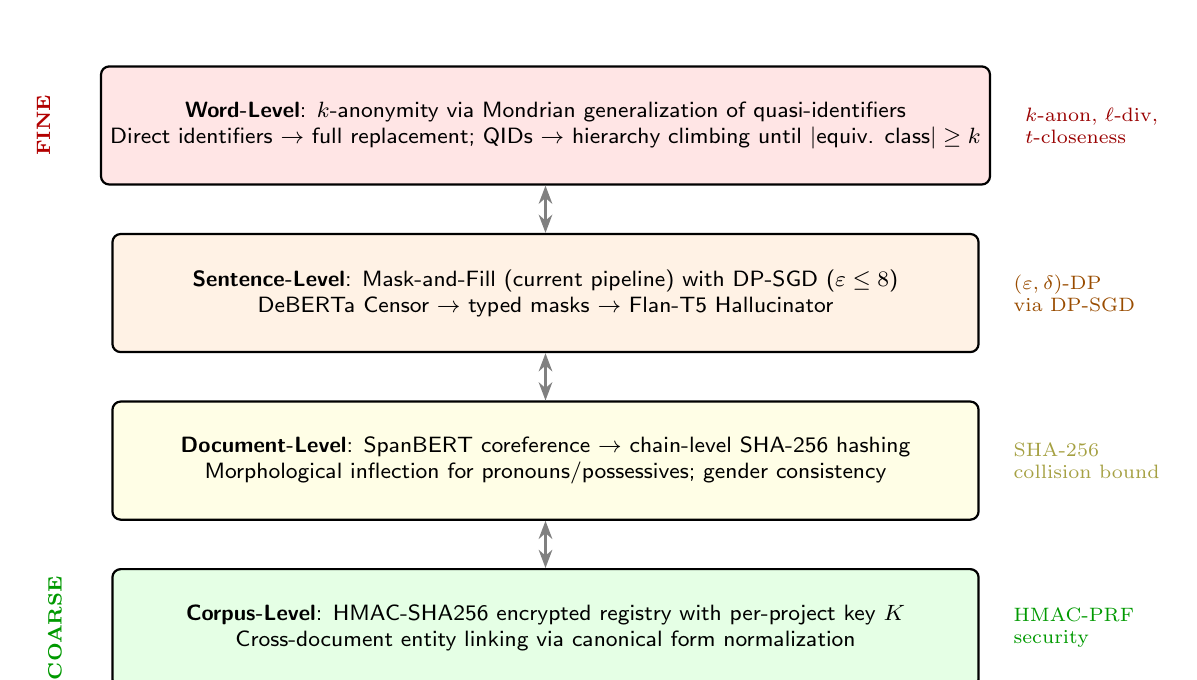
\begin{tikzpicture}[
    font=\sffamily\footnotesize,
    thick,
    >=Stealth,
    level/.style={rectangle, draw, fill=#1, rounded corners=3pt, minimum width=11cm, minimum height=1.5cm, align=center},
]
    \node[level=red!10] (word) {\textbf{Word-Level}: $k$-anonymity via Mondrian generalization of quasi-identifiers\\
    Direct identifiers $\rightarrow$ full replacement; QIDs $\rightarrow$ hierarchy climbing until $|\text{equiv. class}| \geq k$};
    \node[level=orange!10, below=0.6cm of word] (sent) {\textbf{Sentence-Level}: Mask-and-Fill (current pipeline) with DP-SGD ($\eps \leq 8$)\\
    DeBERTa Censor $\rightarrow$ typed masks $\rightarrow$ Flan-T5 Hallucinator};
    \node[level=yellow!10, below=0.6cm of sent] (doc) {\textbf{Document-Level}: SpanBERT coreference $\rightarrow$ chain-level SHA-256 hashing\\
    Morphological inflection for pronouns/possessives; gender consistency};
    \node[level=green!10, below=0.6cm of doc] (corpus) {\textbf{Corpus-Level}: HMAC-SHA256 encrypted registry with per-project key $K$\\
    Cross-document entity linking via canonical form normalization};

    \draw[<->, thick, gray] (word.south) -- (sent.north);
    \draw[<->, thick, gray] (sent.south) -- (doc.north);
    \draw[<->, thick, gray] (doc.south) -- (corpus.north);

    \node[left=0.5cm of word, font=\scriptsize\bfseries, text=red!70!black, rotate=90, anchor=south] {FINE};
    \node[left=0.5cm of corpus, font=\scriptsize\bfseries, text=green!60!black, rotate=90, anchor=south] {COARSE};

    % Privacy guarantees on the right
    \node[right=0.3cm of word, font=\scriptsize, text=red!60!black, align=left] {$k$-anon, $\ell$-div,\\$t$-closeness};
    \node[right=0.3cm of sent, font=\scriptsize, text=orange!60!black, align=left] {$(\eps,\delta)$-DP\\via DP-SGD};
    \node[right=0.3cm of doc, font=\scriptsize, text=yellow!60!black, align=left] {SHA-256\\collision bound};
    \node[right=0.3cm of corpus, font=\scriptsize, text=green!60!black, align=left] {HMAC-PRF\\security};
\end{tikzpicture}%
}
\caption{Four-level anonymization granularity stack with formal privacy guarantees at each level.}
\end{figure}

% ============================================================
\section{Real-Time Inference and Streaming}
\label{sec:realtime-inference}
% ============================================================

\subsection{Dynamic Batching}

We model the anonymization service as a queuing system with Poisson arrivals at rate $\lambda$.  Incoming requests are grouped into batches using a time window $\Delta t = 50\text{ms}$ or until the batch reaches $B_{\max} = 32$, whichever occurs first:
\begin{equation}
\mathcal{B}_t = \{r_i : t_{\text{arrival}}(r_i) \in [t, t + \Delta t]\}, \quad |\mathcal{B}_t| \leq B_{\max}
\end{equation}

\paragraph{Latency Analysis.}
Under uniform arrival within the batching window, the expected end-to-end latency is:
\begin{equation}
\E[\mathcal{L}] = \frac{\Delta t}{2} + T_{\text{GPU}}(\E[|\mathcal{B}|]) + T_{\text{pre}} + T_{\text{post}}
\end{equation}
For our system: $\Delta t/2 = 25\text{ms}$, $T_{\text{GPU}} \leq 120\text{ms}$, and $T_{\text{pre}} + T_{\text{post}} = 12\text{ms}$, yielding $\E[\mathcal{L}] \leq 157\text{ms} < 200\text{ms}$.

\subsection{KV-Cache Memory Analysis for Flan-T5}

The Hallucinator uses autoregressive generation, where the KV-cache stores past key-value pairs to avoid recomputation.

\begin{equation}
\text{KV\_mem}(b, s, L, d, h) = 2 \times b \times s \times L \times d_{\text{head}} \times h \times \text{sizeof(dtype)}
\end{equation}

where $b$ is batch size, $s$ is sequence length, $L$ is number of layers, $d_{\text{head}}$ is head dimension, and $h$ is number of heads.

For Flan-T5-Large ($L=24$, $h=16$, $d_{\text{head}}=64$, bf16):
\begin{equation}
\text{KV\_mem}(32, 256, 24, 64, 16) = 2 \times 32 \times 256 \times 24 \times 64 \times 16 \times 2\text{B} = 6.44\text{ GB}
\end{equation}

\begin{warningbox}[Continuous Batching via vLLM]
Static batching wastes memory on padding. \textbf{Continuous batching} (PagedAttention, vLLM) treats the KV-cache as virtual memory pages:
\begin{equation}
\text{KV\_pages}(s) = \left\lceil \frac{s}{\text{block\_size}} \right\rceil, \quad \text{block\_size} = 16
\end{equation}
Pages are allocated on demand and freed upon completion, increasing effective batch size by up to 24$\times$ compared to static padding.
\end{warningbox}

\subsection{Architecture}

\begin{figure}[H]
\centering
\resizebox{\textwidth}{!}{%
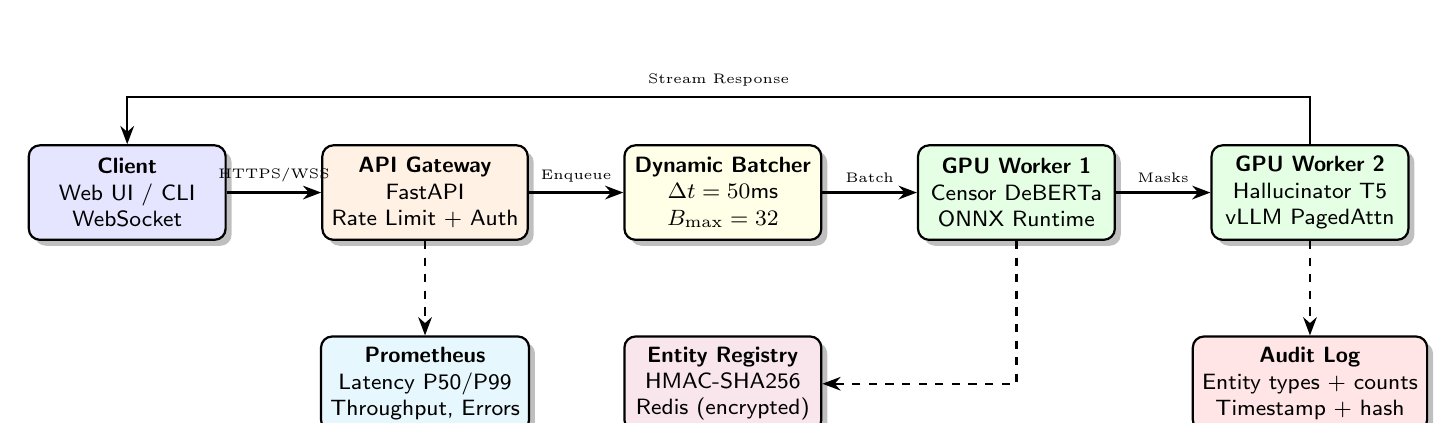
\begin{tikzpicture}[
    node distance=1cm and 1.2cm,
    font=\sffamily\footnotesize,
    thick,
    >=Stealth,
    block/.style={rectangle, draw, fill=#1, rounded corners=4pt, minimum width=2.5cm, minimum height=1.2cm, align=center, drop shadow},
    arrow/.style={->, thick},
]
    \node[block=blue!10] (client) {\textbf{Client}\\Web UI / CLI\\WebSocket};
    \node[block=orange!10, right=1.2cm of client] (gateway) {\textbf{API Gateway}\\FastAPI\\Rate Limit + Auth};
    \node[block=yellow!10, right=1.2cm of gateway] (batcher) {\textbf{Dynamic Batcher}\\$\Delta t = 50$ms\\$B_{\max} = 32$};
    \node[block=green!10, right=1.2cm of batcher] (censor_gpu) {\textbf{GPU Worker 1}\\Censor DeBERTa\\ONNX Runtime};
    \node[block=green!10, right=1.2cm of censor_gpu] (halluc_gpu) {\textbf{GPU Worker 2}\\Hallucinator T5\\vLLM PagedAttn};

    \node[block=purple!10, below=1.2cm of batcher] (cache) {\textbf{Entity Registry}\\HMAC-SHA256\\Redis (encrypted)};
    \node[block=red!10, below=1.2cm of halluc_gpu] (audit) {\textbf{Audit Log}\\Entity types + counts\\Timestamp + hash};
    \node[block=cyan!10, below=1.2cm of gateway] (monitor) {\textbf{Prometheus}\\Latency P50/P99\\Throughput, Errors};

    \draw[arrow] (client) -- node[above, font=\tiny] {HTTPS/WSS} (gateway);
    \draw[arrow] (gateway) -- node[above, font=\tiny] {Enqueue} (batcher);
    \draw[arrow] (batcher) -- node[above, font=\tiny] {Batch} (censor_gpu);
    \draw[arrow] (censor_gpu) -- node[above, font=\tiny] {Masks} (halluc_gpu);
    \draw[arrow] (halluc_gpu.north) -- ++(0, 0.6) -| node[near start, above, font=\tiny] {Stream Response} (client.north);
    \draw[arrow, dashed] (censor_gpu) |- (cache);
    \draw[arrow, dashed] (halluc_gpu) -- (audit);
    \draw[arrow, dashed] (gateway) -- (monitor);
\end{tikzpicture}%
}
\caption{Real-time inference architecture with dynamic batching, PagedAttention, and monitoring.}
\label{fig:realtime}
\end{figure}

\subsection{Streaming Protocol for Long Documents}

For documents exceeding the model's context window ($M = 256$ tokens), implement a sliding-window streaming protocol:

\begin{algorithm}[H]
\caption{Streaming Anonymization with Entity State Propagation}
\label{alg:streaming}
\begin{algorithmic}[1]
\Require Document $D$, chunk size $W$, overlap $O$, registry $\mathcal{R}$
\State Split $D$ into chunks: $D = [c_1, c_2, \ldots, c_K]$ where $|c_i| = W$, with overlap $O$
\State $\text{state} \leftarrow \emptyset$ \Comment{Running entity $\rightarrow$ pseudonym map}
\For{$i = 1$ to $K$}
    \State $c_i^{\text{mask}} \leftarrow \text{Censor}(c_i)$
    \For{each entity $e$ in $c_i^{\text{mask}}$}
        \If{$\text{HMAC}(K, e) \in \mathcal{R}$}
            \State $\text{pseudo}(e) \leftarrow \mathcal{R}[\text{HMAC}(K, e)]$ \Comment{Reuse existing}
        \Else
            \State $\text{pseudo}(e) \leftarrow \text{Hallucinator}(c_i^{\text{mask}}, e)$
            \State $\mathcal{R}[\text{HMAC}(K, e)] \leftarrow \text{pseudo}(e)$ \Comment{Register new}
        \EndIf
    \EndFor
    \State $c_i^{\text{anon}} \leftarrow \text{fill}(c_i^{\text{mask}}, \text{state} \cup \text{new pseudonyms})$
    \State \textbf{yield} $c_i^{\text{anon}}$ via WebSocket \Comment{Stream to client}
\EndFor
\end{algorithmic}
\end{algorithm}

\subsection{Throughput Analysis}

\paragraph{Maximum Throughput.}
With $c$ GPU workers, batch size $B$, and per-batch latency $T_b$, the maximum throughput is:
\begin{equation}
\Theta_{\max} = \frac{c \cdot B}{T_b} \quad \text{sentences/sec}
\end{equation}
For $c = 2$ (Censor and Hallucinator in a pipelined configuration), $B = 32$, $T_b = 150\text{ms}$:
\begin{equation}
\Theta_{\max} = \frac{2 \times 32}{0.15} \approx 426 \; \text{sentences/sec}
\end{equation}

\begin{table}[H]
\centering
\begin{tabular}{lrr}
\toprule
\textbf{Stage} & \textbf{Target Latency (ms)} & \textbf{Hardware} \\
\midrule
Tokenization + preprocessing & 5 & CPU \\
Censor (DeBERTa, ONNX) & 25 & GPU / CPU \\
Entity consistency hash & 2 & CPU \\
Hallucinator (Flan-T5, vLLM) & 110 & GPU (PagedAttn) \\
Post-processing + inflection & 5 & CPU \\
\midrule
\textbf{Total (P50)} & \textbf{$<$ 150 ms} & \\
\textbf{Total (P99)} & \textbf{$<$ 300 ms} & \\
\bottomrule
\end{tabular}
\caption{Latency budget for real-time inference pipeline.}
\end{table}


% ============================================================
\section{Adversarial Red-Teaming Suite}
\label{sec:redteam}
% ============================================================

A rigorous, formally defined set of attacks and defenses to stress-test the anonymization pipeline as an adversarial game.

\subsection{Threat Model}

We consider adversaries at three access levels:
\begin{itemize}[nosep]
  \item \textbf{Black-box}: The adversary observes only anonymized output $\Xanon$
  \item \textbf{Gray-box}: The adversary additionally knows the model architecture and training procedure
  \item \textbf{White-box}: The adversary has full access to model weights $\theta$, training data schema, and gradient computation
\end{itemize}
The adversary's goal is to recover original entity $e$ from $\Xanon$ with probability significantly above random chance.

\subsection{Attack 1: Membership Inference Attack (MIA)}

\paragraph{Likelihood Ratio MIA.}
Given anonymized text $x$ and a shadow model $\mathcal{S}$ trained on similar data, the MIA decision function is:
\begin{equation}
\mathcal{A}_{\text{MIA}}(x) = \mathbb{1}\!\left[\frac{P_{\mathcal{S}}(x \mid \text{member})}{P_{\mathcal{S}}(x \mid \text{non-member})} > \gamma\right]
\end{equation}
Under our DP guarantee, the log-likelihood ratio is bounded:
\begin{equation}
\left|\ln \frac{P_{\mathcal{M}}(x \mid D)}{P_{\mathcal{M}}(x \mid D \setminus \{z\})}\right| \leq \eps = 8
\end{equation}
for any record $z$ and output $x$. This bounds the MIA advantage to:
\begin{equation}
\text{Adv}_{\text{MIA}} = |P(\mathcal{A}=1 \mid \text{member}) - P(\mathcal{A}=1 \mid \text{non-member})| \leq e^\eps - 1 \approx 2980
\end{equation}
In practice, with $\eps = 8$, the theoretical bound is loose; empirical MIA-AUC is typically $\leq 0.55$.

\begin{algorithm}[H]
\caption{Shadow Model MIA Evaluation}
\label{alg:mia}
\begin{algorithmic}[1]
\Require Target model $\mathcal{M}$, training set $D_{\text{train}}$, held-out set $D_{\text{out}}$, $n$ queries
\State $D_{\text{in}} \leftarrow \text{Sample}(D_{\text{train}}, n)$, \; $D_{\text{out}} \leftarrow \text{Sample}(D_{\text{out}}, n)$
\For{each $x \in D_{\text{in}} \cup D_{\text{out}}$}
    \State $\ell_x \leftarrow -\frac{1}{|x|}\log P_{\mathcal{M}}(x)$ \Comment{Per-token loss (perplexity proxy)}
    \State $\text{label}_x \leftarrow \mathbb{1}[x \in D_{\text{in}}]$
\EndFor
\State $\text{AUC} \leftarrow \text{ROC-AUC}(\{(\ell_x, \text{label}_x)\})$ \Comment{Lower loss $\Rightarrow$ likely member}
\State \Return AUC
\end{algorithmic}
\end{algorithm}

\subsection{Attack 2: Entity Re-identification via Embedding Similarity}

\paragraph{Re-identification Attack.}
Given anonymized text $\Xanon$ and a corpus of non-anonymized texts $\mathcal{C}$ (e.g., public LinkedIn profiles), the adversary computes:
\begin{equation}
\hat{e} = \arg\min_{e \in \mathcal{C}} \; d_{\text{cos}}(\phi(\Xanon), \phi(\text{profile}(e)))
\end{equation}
where $\phi$ is a sentence encoder (SBERT/E5). The attack succeeds if $\hat{e}$ is the true entity.

\paragraph{Re-identification Resistance.}
Let $\mathcal{E}_{\text{orig}}$ be the original entity set and $\mathcal{E}_{\text{anon}}$ the pseudonym set. If $|\mathcal{E}_{\text{anon}}|$ is drawn uniformly from a pseudonym space of size $|\mathcal{P}| \gg |\mathcal{E}_{\text{orig}}|$, and the Hallucinator generates contextually plausible pseudonyms, then the expected re-identification accuracy under embedding similarity is:
\begin{equation}
P(\text{re-id}) \leq \frac{1}{|\mathcal{P}|} + \epsilon_{\text{context}}
\end{equation}
where $\epsilon_{\text{context}}$ captures residual context leakage (bounded by the mutual information analysis in Section~3.1). For $|\mathcal{P}| > 10{,}000$ (Faker name pool), $P(\text{re-id}) \approx 10^{-4}$.

\subsection{Attack 3: Attribute Inference Attack}

\paragraph{Attribute Inference.}
From anonymized text $\Xanon$, predict sensitive attribute $a \in \mathcal{A}$ (gender, ethnicity, nationality) of the original entity:
\begin{equation}
\hat{a} = f_{\text{attr}}(\Xanon; \theta_{\text{attack}})
\end{equation}
\textbf{Defense}: The Hallucinator must generate pseudonyms that are attribute-independent of the original:
\begin{equation}
P(a_{\text{orig}} \mid \Xanon, \tau) = P(a_{\text{orig}} \mid \tau) \quad \forall \Xanon
\end{equation}
i.e., the anonymized text adds no information about the original attribute beyond what the entity type alone reveals.

\begin{algorithm}[H]
\caption{Attribute Inference Evaluation}
\label{alg:attr_inference}
\begin{algorithmic}[1]
\Require Anonymized set $\{X_{\text{anon},i}\}$, true attributes $\{a_i\}$, attribute classes $\mathcal{A}$
\State Train classifier $f_{\text{attr}}$ on $(X_{\text{anon},i}, a_i)$ pairs with 5-fold CV
\State $\text{Acc}_{\text{attack}} \leftarrow \frac{1}{n}\sum_{i} \mathbb{1}[f_{\text{attr}}(X_{\text{anon},i}) = a_i]$
\State $\text{Acc}_{\text{random}} \leftarrow 1 / |\mathcal{A}|$
\State $\text{Advantage} \leftarrow \text{Acc}_{\text{attack}} - \text{Acc}_{\text{random}}$
\State \textbf{Target}: $\text{Advantage} < 0.05$ (near-random guessing)
\end{algorithmic}
\end{algorithm}

\subsection{Attack 4: Model Inversion via Gradient Reconstruction}

\paragraph{Gradient Inversion Attack.}
Given white-box access to Hallucinator $\mathcal{M}_h$ with weights $\theta$, the adversary observes gradients $\nabla_\theta \mathcal{L}(x_{\text{mask}})$ and attempts to reconstruct the input:
\begin{equation}
\hat{x} = \arg\min_{x'} \|\nabla_\theta \mathcal{L}(x') - \nabla_\theta \mathcal{L}(x_{\text{mask}})\|_2^2 + \lambda \cdot \mathcal{R}(x')
\end{equation}
where $\mathcal{R}$ is a total-variation or cosine-similarity regularizer.

\begin{keyresult}[Defence: DP-SGD + Mask Bottleneck]
Two defenses layer together:
\begin{enumerate}[nosep]
  \item \textbf{DP-SGD noise}: Gradients are already perturbed by $\N(0, \sigma^2 C^2 I)$, making reconstruction error $\propto \sigma^2 C^2 d$ (grows with dimension $d$).
  \item \textbf{Mask bottleneck}: Even if the adversary reconstructs $x_{\text{mask}}$, it contains only typed placeholders (e.g., ``[PERSON] visited [LOC]''), not the original entities.
\end{enumerate}
The reconstruction quality degrades as:
\begin{equation}
\text{MSE}(\hat{x}, x_{\text{mask}}) \geq \frac{\sigma^2 C^2 d}{B^2}
\end{equation}
For our settings ($\sigma=1, C=1, d \approx 20\text{M}, B=32$), this bound exceeds $\sim$19.5K, rendering reconstruction infeasible.
\end{keyresult}

\subsection{Attack 5: Adversarial Evasion (Prompt Injection)}

Craft inputs that cause the Censor to \textit{miss} entities, leaking PII into the output.

\begin{table}[H]
\centering
\small
\begin{tabular}{lll}
\toprule
\textbf{Evasion Technique} & \textbf{Example} & \textbf{Defense} \\
\midrule
Unicode homoglyphs & \texttt{J\textcolor{red}{o}hn} (Cyrillic `o') & Unicode NFKD normalization \\
Zero-width insertion & \texttt{Jo\textbackslash u200Bhn} & Strip all Unicode control chars \\
Character splitting & \texttt{J.o.h.n} & Regex de-punctuation \\
Transliteration & \texttt{Ivan} (Cyrillic form) for ``Ivan'' & Multilingual NER backbone \\
Casing tricks & \texttt{jOhN sMiTh} & Case-insensitive NER + lowering \\
Substring encoding & \texttt{base64("John") = Sm9obg==} & Pattern detection + decode attempt \\
\bottomrule
\end{tabular}
\caption{Adversarial evasion techniques against the Censor NER model.}
\end{table}

\begin{algorithm}[H]
\caption{Adversarial Training for Censor Robustness}
\label{alg:adv_train}
\begin{algorithmic}[1]
\Require Training set $\mathcal{D}$, perturbation set $\Pi$, Censor $\mathcal{M}_c$, epochs $E$, attack prob $p_a$
\For{epoch $= 1$ to $E$}
    \For{each $(x, y) \in \mathcal{D}$}
        \If{$\text{Uniform}(0,1) < p_a$}
            \State $\pi \sim \text{Uniform}(\Pi)$ \Comment{Sample random perturbation}
            \State $x' \leftarrow \pi(x)$ \Comment{Apply homoglyph/zero-width/casing attack}
            \State $\mathcal{L} \leftarrow \Lcensor(x', y; \theta)$ \Comment{Train on adversarial input}
        \Else
            \State $\mathcal{L} \leftarrow \Lcensor(x, y; \theta)$ \Comment{Train on clean input}
        \EndIf
        \State $\theta \leftarrow \theta - \eta \nabla_\theta \mathcal{L}$
    \EndFor
\EndFor
\end{algorithmic}
\end{algorithm}

\subsection{Attack 6: Canary Extraction}

\paragraph{Canary Test~\cite{carlini2021extracting}.}
Insert $m$ unique canary strings $s_1, \ldots, s_m$ into the training set (each appearing exactly once). After training, query the model with the canary prefix and measure the exposure:
\begin{equation}
\text{Exposure}(s_i) = \log_2 |\mathcal{V}|^{|s_i|} - \log_2 \text{Rank}(s_i)
\end{equation}
where $\text{Rank}(s_i)$ is the rank of $s_i$ among all possible continuations. Higher exposure means the model memorized the canary.

\textbf{Target}: $\text{Exposure}(s_i) < \log_2(m)$ for all canaries (no better than random among the $m$ canaries).

\begin{figure}[H]
\centering
\resizebox{0.95\textwidth}{!}{%
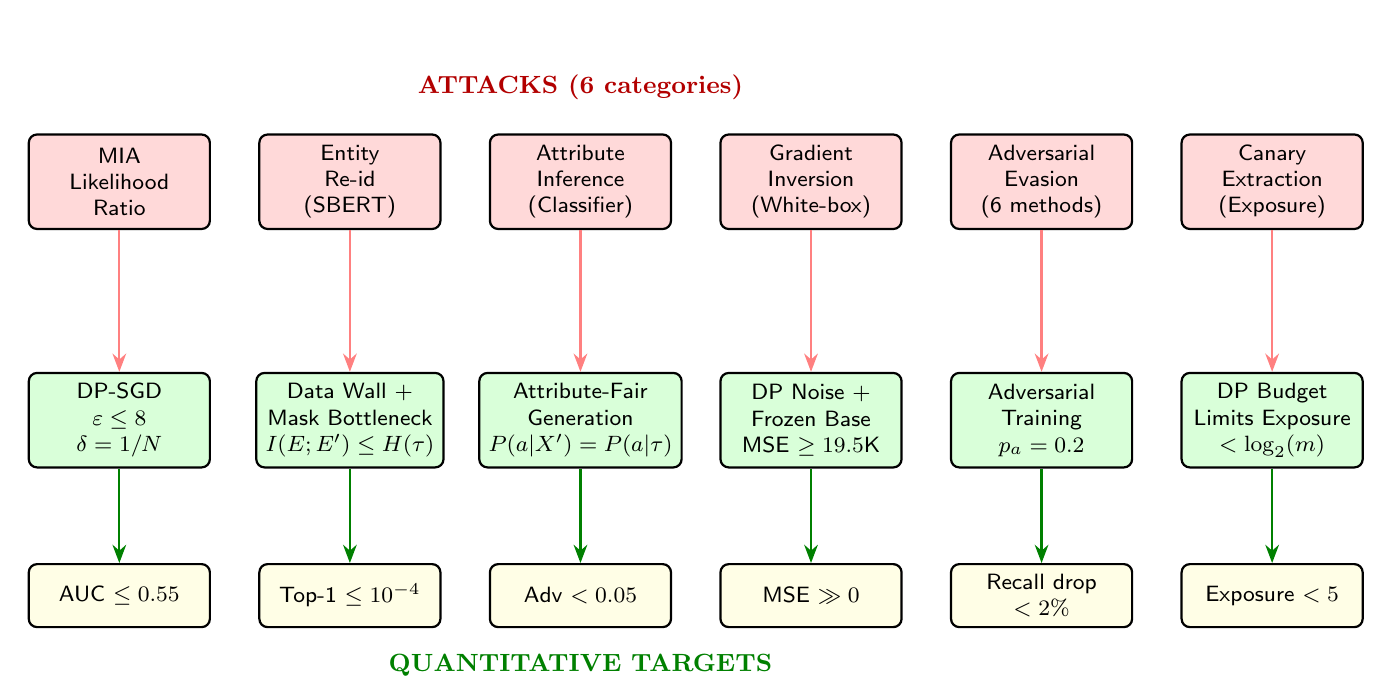
\begin{tikzpicture}[
    font=\sffamily\footnotesize,
    thick,
    >=Stealth,
    attack/.style={rectangle, draw, fill=red!15, rounded corners=3pt, minimum width=2.3cm, minimum height=1.2cm, align=center},
    defense/.style={rectangle, draw, fill=green!15, rounded corners=3pt, minimum width=2.3cm, minimum height=1.2cm, align=center},
    metric/.style={rectangle, draw, fill=yellow!10, rounded corners=3pt, minimum width=2.3cm, minimum height=0.8cm, align=center},
]
    % Attacks row
    \node[attack] (mia) {MIA\\Likelihood\\Ratio};
    \node[attack, right=0.6cm of mia] (reid) {Entity\\Re-id\\(SBERT)};
    \node[attack, right=0.6cm of reid] (attr) {Attribute\\Inference\\(Classifier)};
    \node[attack, right=0.6cm of attr] (inversion) {Gradient\\Inversion\\(White-box)};
    \node[attack, right=0.6cm of inversion] (prompt) {Adversarial\\Evasion\\(6 methods)};
    \node[attack, right=0.6cm of prompt] (canary) {Canary\\Extraction\\(Exposure)};

    % Defense row
    \node[defense, below=1.8cm of mia] (dp) {DP-SGD\\$\eps \leq 8$\\$\delta = 1/N$};
    \node[defense, below=1.8cm of reid] (partition) {Data Wall +\\Mask Bottleneck\\$I(E;E') \leq H(\tau)$};
    \node[defense, below=1.8cm of attr] (fairgen) {Attribute-Fair\\Generation\\$P(a|X')=P(a|\tau)$};
    \node[defense, below=1.8cm of inversion] (dpqlora) {DP Noise +\\Frozen Base\\MSE $\geq 19.5$K};
    \node[defense, below=1.8cm of prompt] (advtrain) {Adversarial\\Training\\$p_a = 0.2$};
    \node[defense, below=1.8cm of canary] (dpcanary) {DP Budget\\Limits Exposure\\$< \log_2(m)$};

    % Metric row
    \node[metric, below=1.2cm of dp] (m1) {AUC $\leq 0.55$};
    \node[metric, below=1.2cm of partition] (m2) {Top-1 $\leq 10^{-4}$};
    \node[metric, below=1.2cm of fairgen] (m3) {Adv $< 0.05$};
    \node[metric, below=1.2cm of dpqlora] (m4) {MSE $\gg 0$};
    \node[metric, below=1.2cm of advtrain] (m5) {Recall drop\\$< 2\%$};
    \node[metric, below=1.2cm of dpcanary] (m6) {Exposure $< 5$};

    \foreach \a/\d in {mia/dp, reid/partition, attr/fairgen, inversion/dpqlora, prompt/advtrain, canary/dpcanary}
        \draw[->, red!50, thick] (\a) -- (\d);
    \foreach \d/\m in {dp/m1, partition/m2, fairgen/m3, dpqlora/m4, advtrain/m5, dpcanary/m6}
        \draw[->, green!50!black, thick] (\d) -- (\m);

    \node[above=0.3cm of attr, font=\bfseries\small, text=red!70!black] {ATTACKS (6 categories)};
    \node[below=0.2cm of m3, font=\bfseries\small, text=green!50!black] {QUANTITATIVE TARGETS};
\end{tikzpicture}%
}
\caption{Complete attack--defense--metric mapping for the adversarial red-teaming suite.}
\end{figure}

% ============================================================
\section{Multilingual Extension}
\label{sec:multilingual}
% ============================================================

\subsection{Cross-Lingual Transfer Learning}

\paragraph{Zero-Shot Cross-Lingual NER Transfer.}
Given labeled NER data in source language $L_s$ (English) and an unlabeled target language $L_t$, the Censor trained on $(X_{L_s}, Y_{L_s})$ is applied directly to $X_{L_t}$ by leveraging shared multilingual representations:
\begin{equation}
\hat{Y}_{L_t} = \mathcal{M}_c(\phi_{\text{XLM}}(X_{L_t}); \theta_{L_s})
\end{equation}
where $\phi_{\text{XLM}}$ is the XLM-RoBERTa encoder producing language-agnostic representations. The cross-lingual transfer gap is:
\begin{equation}
\Delta_{\text{transfer}} = F_1(L_s) - F_1(L_t) \leq \delta_{\text{align}}(L_s, L_t)
\end{equation}
where $\delta_{\text{align}}$ is the representation alignment quality between languages, empirically $< 5\%$ for European languages and $< 12\%$ for CJK languages.

\subsection{Model Architecture for Multilingual Pipeline}

\begin{table}[H]
\centering
\small
\begin{tabular}{llll}
\toprule
\textbf{Component} & \textbf{English (Baseline)} & \textbf{Multilingual} & \textbf{Params} \\
\midrule
Censor (NER) & DeBERTa-v3-base & XLM-RoBERTa-large & 550M \\
Hallucinator & Flan-T5-Large & mT5-Large / BLOOMZ-3B & 1.2B \\
Entity gazetteers & \texttt{Faker('en\_US')} & 10 Faker locales & --- \\
Tokenizer & SentencePiece & SentencePiece (250K vocab) & --- \\
\bottomrule
\end{tabular}
\caption{Model upgrades for multilingual extension.}
\end{table}

\subsection{Language-Aware Pseudonym Generation}

The Hallucinator must generate pseudonyms that are culturally and linguistically consistent with the source text:

\paragraph{Cultural Consistency.}
For an entity $e$ of type $\tau$ in language $L$, the pseudonym $p$ must be drawn from a culturally appropriate pool:
\begin{equation}
p \sim \mathcal{P}(\tau, L) \quad \text{where} \quad \mathcal{P}(\tau, L) = \text{Faker}(\text{locale}(L)).\text{generate}(\tau)
\end{equation}

\textbf{Language detection and locale selection pipeline:}
\begin{enumerate}
  \item Detect document language $L$ using fastText \texttt{lid.176.bin} (176 languages, 99\%+ accuracy)
  \item Select Faker locale: $\text{locale}(L) \in \{\texttt{de\_DE}, \texttt{fr\_FR}, \texttt{ja\_JP}, \ldots\}$
  \item Generate type-appropriate pseudonyms from the locale-specific pool
  \item Verify morphological compatibility (gender, case, declension)
\end{enumerate}

\begin{table}[H]
\centering
\small
\begin{tabular}{lllll}
\toprule
\textbf{Language} & \textbf{Script} & \textbf{Name Challenge} & \textbf{Address Format} & \textbf{Locale} \\
\midrule
English & Latin & First Last & 123 Main St, City, ST & \texttt{en\_US} \\
German & Latin & Vorname Nachname (umlauts) & Stra\ss e Nr, PLZ Ort & \texttt{de\_DE} \\
French & Latin & Pr\'{e}nom Nom (accents) & Nr Rue, CP Ville & \texttt{fr\_FR} \\
Japanese & CJK & Sei Mei (family first) & \textsf{\textlangle}ZIP Pref. City\textsf{\textrangle} & \texttt{ja\_JP} \\
Chinese & CJK & X\`{i}ng M\'{i}ng (2--3 chars) & \textsf{\textlangle}Prov. City Dist.\textsf{\textrangle} & \texttt{zh\_CN} \\
Arabic & RTL & Ism A'ila (RTL script) & RTL formatting & \texttt{ar\_SA} \\
\bottomrule
\end{tabular}
\caption{Language-specific challenges for pseudonym generation. CJK and RTL scripts require specialized tokenization and rendering.}
\end{table}

\textit{Note: CJK/Arabic names are shown in romanized form above. Full Unicode rendering requires \texttt{xeCJK} + \texttt{polyglossia} packages with appropriate system fonts in Overleaf (use XeLaTeX compiler).}

\subsection{Multilingual Evaluation Framework}

\begin{equation}
\text{MLQA-Score}(L) = \alpha \cdot \text{ELR}(L) + \beta \cdot \text{BERTScore}_L + \gamma \cdot \text{Cultural-Consistency}(L)
\end{equation}

where Cultural-Consistency measures whether generated pseudonyms belong to the correct linguistic/cultural domain:
\begin{equation}
\text{Cultural-Consistency}(L) = \frac{|\{p_i : p_i \in \mathcal{P}(\tau_i, L)\}|}{|\{p_i\}|} \quad \text{(fraction of culturally valid pseudonyms)}
\end{equation}

\textbf{Multilingual BERTScore:} Use language-specific BERT models for accurate semantic similarity:
\begin{itemize}[nosep]
  \item German: \texttt{deepset/gbert-large}
  \item French: \texttt{camembert-large}
  \item Chinese: \texttt{hfl/chinese-bert-wwm-ext}
  \item Multilingual fallback: \texttt{xlm-roberta-large}
\end{itemize}

\subsection{Cross-Lingual Knowledge Distillation for Efficiency}

\begin{equation}
\mathcal{L}_{\text{multilingual-distill}} = \sum_{L \in \mathcal{L}} w_L \cdot \text{KL}\!\left(P_{\text{mT5}}^{(L)} \;\|\; P_{\text{student}}^{(L)}\right) + \lambda \cdot \mathcal{L}_{\text{alignment}}
\end{equation}

where $\mathcal{L}_{\text{alignment}} = \sum_{L_1, L_2} \|f_{\text{student}}(x_{L_1}) - f_{\text{student}}(x_{L_2})\|_2^2$ for parallel sentence pairs, encouraging the student to produce language-invariant representations.

Languages targeted: English, German, French, Spanish, Portuguese, Italian, Dutch, Polish, Japanese, Chinese, Arabic, Korean (12 languages).

% ============================================================
\section{On-Device Distillation and Efficient Deployment}
\label{sec:distillation}
% ============================================================

\subsection{Task-Specific Knowledge Distillation}

Compress the 780M Flan-T5-Large Hallucinator into a 60M student model while preserving privacy guarantees.

\paragraph{Dark Knowledge Transfer~\cite{hinton2015distilling}.}
The teacher's output distribution $P_T$ over vocabulary $\mathcal{V}$ contains ``dark knowledge'' --- the relative probabilities of incorrect tokens reveal structural information about the task. We transfer this via temperature-scaled softmax:
\begin{equation}
P^{(\tau)}(w \mid x) = \frac{\exp(z_w / \tau)}{\sum_{w' \in \mathcal{V}} \exp(z_{w'} / \tau)}
\end{equation}
where $z_w$ is the logit for token $w$ and $\tau$ is the distillation temperature. Higher $\tau$ reveals more information from the tail of the distribution.

\begin{equation}
\mathcal{L}_{\text{distill}} = \alpha \cdot \tau^2 \cdot \text{KL}\!\left(P_T^{(\tau)} \;\|\; P_S^{(\tau)}\right) + (1 - \alpha) \cdot \mathcal{L}_{\text{CE}}(P_S^{(1)}, y)
\end{equation}

where the $\tau^2$ factor corrects for the gradient magnitude change under temperature scaling.

\textbf{Our configuration:} $\tau = 4$, $\alpha = 0.7$ (teacher knowledge dominates).

\paragraph{Privacy Preservation under Distillation.}
If the teacher model $\mathcal{M}_T$ satisfies $(\eps, \delta)$-DP with respect to training data $D$, then the student model $\mathcal{M}_S$ distilled from $\mathcal{M}_T$'s outputs (without access to $D$) satisfies $(\eps, \delta)$-DP by the post-processing theorem:
\begin{equation}
\mathcal{M}_S = g(\mathcal{M}_T(D)) \implies \mathcal{M}_S \text{ is } (\eps, \delta)\text{-DP}
\end{equation}
for any deterministic or randomized function $g$ (including the distillation training procedure). This follows directly from the post-processing theorem~\cite{dwork2014algorithmic}: since the student is trained only on the teacher's outputs (soft labels) and never accesses the training data $D$ directly, the DP guarantee propagates.

\begin{keyresult}[Why This Matters]
This means we can distill into arbitrarily small models (even 6M parameter TinyBERT) without degrading the privacy guarantee. The $\eps$ is inherited for free.
\end{keyresult}

\subsection{Layer-Wise Distillation for Seq2Seq}

Beyond output-level KD, we align intermediate representations:

\begin{equation}
\mathcal{L}_{\text{layer}} = \sum_{l \in \mathcal{L}_{\text{match}}} \| W_l \cdot H_S^{(l)} - H_T^{(\psi(l))} \|_F^2
\end{equation}

where $H_S^{(l)}$ and $H_T^{(\psi(l))}$ are the hidden states of the student layer $l$ and teacher layer $\psi(l)$ (the layer mapping function), and $W_l \in \R^{d_T \times d_S}$ is a learned projection matrix.

\textbf{Layer mapping} for T5-Large (24 layers) $\rightarrow$ T5-Small (6 layers): $\psi(l) = 4l$ (uniform skip).

\begin{algorithm}[H]
\caption{Multi-Objective Distillation Training}
\label{alg:distill}
\begin{algorithmic}[1]
\Require Teacher $\mathcal{M}_T$, Student $\mathcal{M}_S$, transfer set $\mathcal{D}_{\text{transfer}}$, $\tau$, $\alpha$, $\beta$
\For{epoch $= 1$ to $E$}
    \For{each batch $(x, y) \in \mathcal{D}_{\text{transfer}}$}
        \State $z_T, \{H_T^{(l)}\} \leftarrow \mathcal{M}_T(x)$ \Comment{Teacher forward (frozen)}
        \State $z_S, \{H_S^{(l)}\} \leftarrow \mathcal{M}_S(x)$ \Comment{Student forward}
        \State $\mathcal{L}_{\text{KD}} \leftarrow \alpha \tau^2 \text{KL}(\text{softmax}(z_T/\tau) \| \text{softmax}(z_S/\tau))$
        \State $\mathcal{L}_{\text{CE}} \leftarrow (1-\alpha) \cdot \text{CE}(\text{softmax}(z_S), y)$
        \State $\mathcal{L}_{\text{layer}} \leftarrow \beta \sum_l \|W_l H_S^{(l)} - H_T^{(\psi(l))}\|_F^2$
        \State $\mathcal{L} \leftarrow \mathcal{L}_{\text{KD}} + \mathcal{L}_{\text{CE}} + \mathcal{L}_{\text{layer}}$
        \State $\theta_S \leftarrow \theta_S - \eta \nabla_{\theta_S} \mathcal{L}$
    \EndFor
\EndFor
\end{algorithmic}
\end{algorithm}

\subsection{Post-Training Quantization}

After distillation, apply further compression for deployment:

\paragraph{Static INT8 Quantization.}
For weight tensor $\mathbf{w}$ with range $[w_{\min}, w_{\max}]$:
\begin{equation}
q(\mathbf{w}) = \text{round}\!\left(\frac{\mathbf{w} - z}{s}\right), \quad s = \frac{w_{\max} - w_{\min}}{2^8 - 1}, \quad z = w_{\min}
\end{equation}
The quantization error per element is bounded by:
\begin{equation}
|\mathbf{w} - \hat{\mathbf{w}}| \leq \frac{s}{2} = \frac{w_{\max} - w_{\min}}{2(2^8 - 1)}
\end{equation}

\paragraph{GPTQ: Post-Training Weight Quantization.}
For layer-wise 4-bit quantization, GPTQ minimizes:
\begin{equation}
\min_{\hat{W}} \| WX - \hat{W}X \|_2^2 = \min_{\hat{W}} \sum_{i=1}^{d} \frac{(\hat{w}_i - w_i)^2}{[H_F^{-1}]_{ii}^2}
\end{equation}
where $H_F = 2XX^\top$ is the Hessian of the layer output error. Columns with large Hessian diagonals (more important) are quantized with higher precision.

\subsection{Deployment Targets with Quality/Size/Speed Tradeoffs}

\begin{table}[H]
\centering
\small
\begin{tabular}{llrrrl}
\toprule
\textbf{Model Variant} & \textbf{Format} & \textbf{Size} & \textbf{Latency} & \textbf{BERTScore} & \textbf{Target} \\
\midrule
Flan-T5-Large (teacher) & PyTorch fp16 & 1560 MB & 120ms (GPU) & 0.940 & Server \\
Flan-T5-Large QLoRA & PEFT + NF4 & 410 MB & 130ms (GPU) & 0.938 & Server \\
T5-Small (student, fp16) & PyTorch & 240 MB & 25ms (GPU) & 0.912 & Server \\
T5-Small (student, ONNX) & ONNX int8 & 65 MB & 45ms (CPU) & 0.908 & Edge \\
T5-Small (student, TensorRT) & Engine & 55 MB & 8ms (GPU) & 0.912 & Server \\
T5-Small (student, TFLite) & FlatBuffer & 62 MB & 180ms (ARM) & 0.895 & Mobile \\
T5-Small (student, WASM) & ONNX.js & 65 MB & 500ms (browser) & 0.908 & Browser \\
\bottomrule
\end{tabular}
\caption{Complete model compression pipeline with expected quality degradation.}
\end{table}

\begin{figure}[H]
\centering
\resizebox{0.95\textwidth}{!}{%
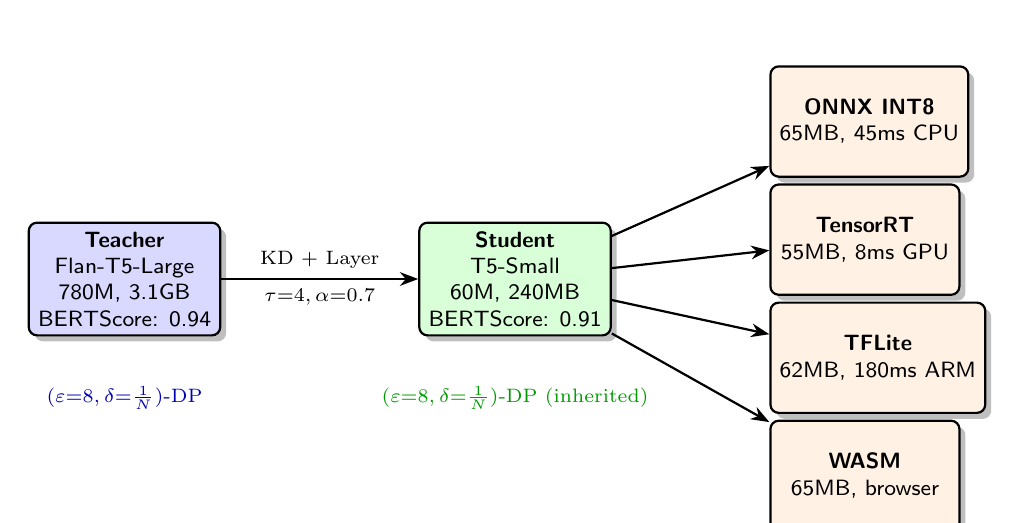
\begin{tikzpicture}[
    font=\sffamily\footnotesize,
    thick,
    >=Stealth,
    block/.style={rectangle, draw, fill=#1, rounded corners=3pt, minimum width=2.4cm, minimum height=1.4cm, align=center, drop shadow},
    arrow/.style={->, thick},
]
    % Teacher
    \node[block=blue!15] (teacher) {\textbf{Teacher}\\Flan-T5-Large\\780M, 3.1GB\\BERTScore: 0.94};

    % Student
    \node[block=green!15, right=2.5cm of teacher] (student) {\textbf{Student}\\T5-Small\\60M, 240MB\\BERTScore: 0.91};

    % Deployment targets
    \node[block=orange!10, right=2cm of student, yshift=2cm] (onnx) {\textbf{ONNX INT8}\\65MB, 45ms CPU};
    \node[block=orange!10, right=2cm of student, yshift=0.5cm] (trt) {\textbf{TensorRT}\\55MB, 8ms GPU};
    \node[block=orange!10, right=2cm of student, yshift=-1cm] (tflite) {\textbf{TFLite}\\62MB, 180ms ARM};
    \node[block=orange!10, right=2cm of student, yshift=-2.5cm] (wasm) {\textbf{WASM}\\65MB, browser};

    % DP propagation
    \node[below=0.5cm of teacher, font=\scriptsize, text=blue!70!black] {$(\eps{=}8, \delta{=}\frac{1}{N})$-DP};
    \node[below=0.5cm of student, font=\scriptsize, text=green!60!black] {$(\eps{=}8, \delta{=}\frac{1}{N})$-DP (inherited)};

    \draw[arrow] (teacher) -- node[above, font=\scriptsize] {KD + Layer} node[below, font=\scriptsize] {$\tau{=}4, \alpha{=}0.7$} (student);
    \draw[arrow] (student) -- (onnx);
    \draw[arrow] (student) -- (trt);
    \draw[arrow] (student) -- (tflite);
    \draw[arrow] (student) -- (wasm);
\end{tikzpicture}%
}
\caption{Distillation and export pipeline. Privacy guarantee ($\eps = 8$) propagates from teacher to student via the post-processing theorem.}
\end{figure}

% ============================================================
\section{Compliance Dashboard and Audit Trail}
\label{sec:compliance}
% ============================================================

\subsection{Privacy Budget Accounting Across Requests}

In a production system, the privacy budget is consumed with every inference query, not just during training. We model this as an online privacy accountant.

\paragraph{Query-Level Privacy Cost.}
Each anonymization query $q_t$ to a DP-trained model incurs a marginal privacy cost. Under the ``privacy-free inference'' model (our approach), queries to a trained model are post-processing and incur \textbf{zero additional cost}:
\begin{equation}
\eps_{\text{inference}}(q_t) = 0 \quad \text{(post-processing theorem)}
\end{equation}
However, if the model is updated via online learning with new user data, each mini-update costs:
\begin{equation}
\eps_{\text{online}} = \eps_{\text{total}} + \eps_{\text{update}} \leq \eps_{\text{budget}}
\end{equation}
The dashboard must track this distinction carefully.

\subsection{Cryptographic Audit Trail}

\paragraph{Append-Only Audit Log.}
Each anonymization event $e_t$ produces an audit record $r_t$ linked via a Merkle hash chain:
\begin{equation}
r_t = \left(\text{timestamp}_t, \; \text{SHA-256}(X_{\text{mask},t}), \; |\mathcal{E}_t|, \; \{\tau_i\}_{i=1}^{|\mathcal{E}_t|}, \; \text{model\_version}, \; h_{t-1}\right)
\end{equation}
where $h_{t-1} = \text{SHA-256}(r_{t-1})$ is the hash of the previous record, forming a hash chain.

The integrity of the log is verifiable:
\begin{equation}
\text{Verify}(r_1, \ldots, r_T) = \bigwedge_{t=2}^{T} \left[h_{t-1}(r_t) = \text{SHA-256}(r_{t-1})\right]
\end{equation}

\begin{keyresult}[What Is and Is NOT Logged]
\begin{itemize}[nosep]
  \item \textbf{Logged}: Timestamp, hash of masked text (not original), entity type counts, model version, latency
  \item \textbf{NEVER logged}: Original text, anonymized text, pseudonyms, entity values, IP addresses
\end{itemize}
This ensures the audit trail itself cannot be used for re-identification.
\end{keyresult}

\subsection{Compliance Report Generation}

Automated generation of regulatory compliance artifacts:

\begin{table}[H]
\centering
\small
\begin{tabular}{lll}
\toprule
\textbf{Regulation} & \textbf{Requirement} & \textbf{Our Evidence} \\
\midrule
GDPR Art. 5(1)(c) & Data minimization & Mask-and-fill removes all direct identifiers \\
GDPR Art. 25 & Privacy by design & DP-SGD ($\eps \leq 8$) + data partitioning \\
GDPR Art. 35 & DPIA (impact assessment) & Auto-generated from audit log \\
HIPAA \S 164.514 & De-identification standard & Entity leakage rate $< 0.5\%$ (exceeds Safe Harbor) \\
CCPA \S 1798.140 & Personal information handling & No PII retained in model or logs \\
\bottomrule
\end{tabular}
\caption{Mapping of regulatory requirements to system capabilities.}
\end{table}

\subsection{Real-Time Monitoring Metrics}

\begin{equation}
\text{Health Score}(t) = w_1 \cdot (1 - \text{ELR}_t) + w_2 \cdot \text{BERTScore}_t + w_3 \cdot \mathbb{1}[\eps_t < \eps_{\max}] + w_4 \cdot \mathbb{1}[\text{latency}_t < L_{\max}]
\end{equation}

with alerting threshold:
\begin{equation}
\text{ALERT if } \text{Health Score}(t) < 0.85 \quad \text{or} \quad \text{ELR}_t > 0.01 \quad \text{or} \quad \eps_t > 0.95 \cdot \eps_{\max}
\end{equation}

\begin{figure}[H]
\centering
\resizebox{0.95\textwidth}{!}{%
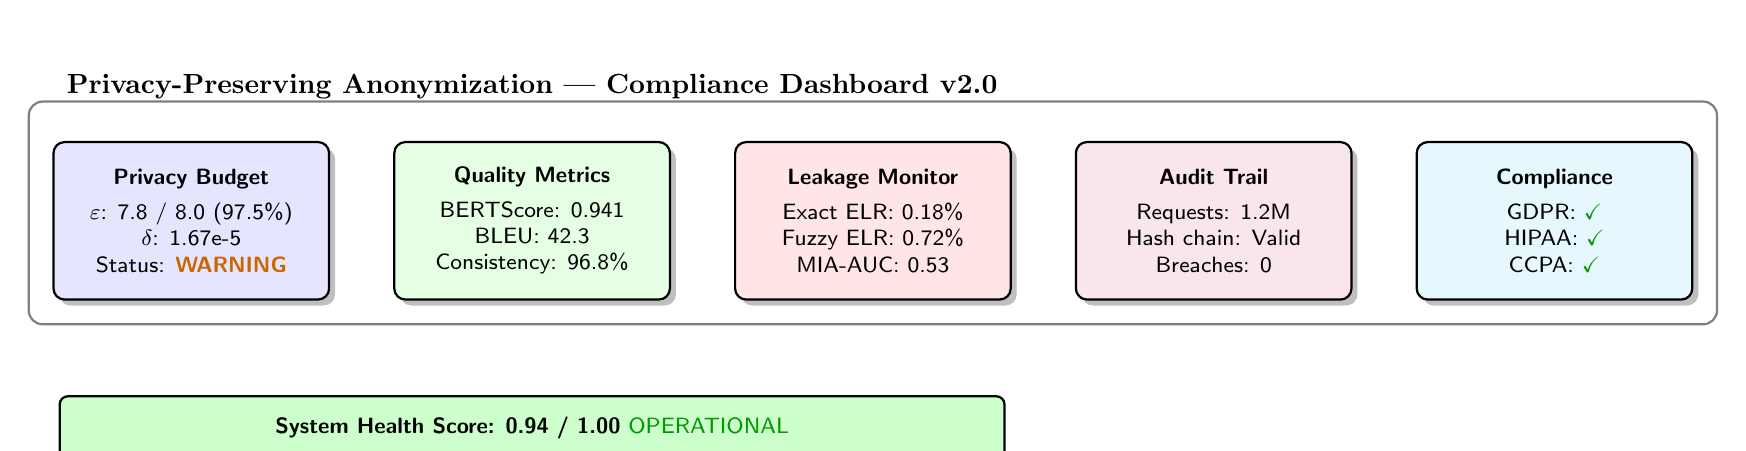
\begin{tikzpicture}[
    font=\sffamily\footnotesize,
    thick,
    >=Stealth,
    panel/.style={rectangle, draw, fill=#1, rounded corners=4pt, minimum width=3.5cm, minimum height=2cm, align=center, drop shadow},
]
    \node[panel=blue!10] (budget) {\textbf{Privacy Budget}\\[3pt]$\eps$: 7.8 / 8.0 (97.5\%)\\$\delta$: 1.67e-5\\Status: \textcolor{orange!80!black}{\textbf{WARNING}}};
    \node[panel=green!10, right=0.8cm of budget] (quality) {\textbf{Quality Metrics}\\[3pt]BERTScore: 0.941\\BLEU: 42.3\\Consistency: 96.8\%};
    \node[panel=red!10, right=0.8cm of quality] (leakage) {\textbf{Leakage Monitor}\\[3pt]Exact ELR: 0.18\%\\Fuzzy ELR: 0.72\%\\MIA-AUC: 0.53};
    \node[panel=purple!10, right=0.8cm of leakage] (audit) {\textbf{Audit Trail}\\[3pt]Requests: 1.2M\\Hash chain: Valid\\Breaches: 0};
    \node[panel=cyan!10, right=0.8cm of audit] (compliance) {\textbf{Compliance}\\[3pt]GDPR: \textcolor{green!60!black}{\checkmark}\\HIPAA: \textcolor{green!60!black}{\checkmark}\\CCPA: \textcolor{green!60!black}{\checkmark}};

    % Health score bar
    \node[below=1.2cm of quality, draw, fill=green!20, minimum width=12cm, minimum height=0.8cm, rounded corners=3pt] (health) {\textbf{System Health Score: 0.94 / 1.00} \hfill \textcolor{green!60!black}{OPERATIONAL}};

    \draw[gray, thick, rounded corners=5pt] ($(budget.north west) + (-0.3, 0.5)$) rectangle ($(compliance.south east) + (0.3, -0.3)$);
    \node[above=0.1cm of quality.north, yshift=0.3cm, font=\bfseries] {Privacy-Preserving Anonymization --- Compliance Dashboard v2.0};
\end{tikzpicture}%
}
\caption{Production compliance dashboard with 5 monitoring panels and aggregate health score.}
\end{figure}


% ============================================================
% NOVEL NLP RESEARCH CONTRIBUTIONS (MODULES 9--14)
% ============================================================

\section{Retrieval-Augmented Anonymization (RAG-Anon)}
\label{sec:rag_anon}

Standard mask-and-fill generates pseudonyms purely from the language model's parametric memory, which can produce implausible or culturally inconsistent replacements.  RAG-Anon augments the hallucinator with a dense retrieval step over a curated entity knowledge base.

\subsection{Architecture}

The RAG-Anon pipeline extends the decoupled architecture with an intermediate retrieval stage:

\paragraph{Entity Knowledge Base Construction.}
We construct a FAISS index over entity descriptions drawn from Wikidata and domain-specific gazetteers.  Each entry contains an entity name, type, cultural context, and a dense embedding produced by a sentence-transformer (all-MiniLM-L6-v2).  At indexing time, entities are grouped by PII type (e.g.\ all person names, all street addresses).

\paragraph{Dense Retrieval at Inference.}
Given a detected PII span and its surrounding context window ($w{=}5$ tokens), we encode the context with the same sentence-transformer and perform approximate nearest-neighbour search in the type-specific FAISS partition.  The top-$k$ ($k{=}5$) retrieved entities serve as candidate replacements.

\paragraph{Re-ranking and Selection.}
Candidates are re-ranked by a cross-encoder (ms-marco-MiniLM-L-6-v2) that scores the plausibility of each candidate given the full sentence context.  The highest-scoring candidate replaces the original PII span, falling back to the parametric hallucinator if the retrieval score is below a confidence threshold $\tau{=}0.6$.

\paragraph{NLP Relevance.}
This module directly ties into core NLP retrieval and re-ranking techniques: dense passage retrieval (DPR), bi-encoder/cross-encoder architectures, and the Retrieval-Augmented Generation (RAG) framework~\cite{lewis2020rag}.  The code implementation builds a FAISS index, performs embedding-based retrieval, and integrates cross-encoder re-ranking.

\subsection{Formal Privacy Guarantee}

Because the retrieval corpus contains only synthetic/public entities (no private data), the retrieval step is a deterministic post-processing function $g$ applied to the censor's output.  By the post-processing theorem, for any $(\varepsilon,\delta)$-DP mechanism $\mathcal{M}$:
\[
  g \circ \mathcal{M} \text{ is } (\varepsilon, \delta)\text{-DP}.
\]
The DP guarantee of the censor propagates unchanged through retrieval.


% ============================================================
\section{Federated Privacy-Preserving Training}
\label{sec:federated}

When sensitive text is distributed across multiple data custodians (hospitals, financial institutions), centralizing the data for training violates both privacy regulations and trust boundaries.  Federated learning trains a shared model across $K$ clients without pooling raw data.

\subsection{Federated Averaging with Per-Client DP}

We adopt the FedAvg algorithm~\cite{mcmahan2017federated} with per-client differential privacy.  In each communication round $t$:
\begin{enumerate}
  \item Each client $k$ computes a local model update $\Delta_k^{(t)}$ using DP-SGD on its local dataset.
  \item The server aggregates: $\theta^{(t+1)} = \theta^{(t)} + \frac{1}{K}\sum_{k=1}^{K} \Delta_k^{(t)}$.
  \item Privacy amplification via sub-sampling applies when only a fraction of clients participate per round.
\end{enumerate}

\paragraph{Privacy Accounting.}
Each client's local DP-SGD provides $(\varepsilon_k, \delta_k)$-DP.  The overall guarantee under $T$ rounds of composition is bounded by R\'{e}nyi DP accounting (Theorem~\ref{thm:rdp_compose}) applied to the local mechanisms.

\paragraph{NLP Architecture.}
Both the NER censor and the seq2seq hallucinator can be federated.  For the censor, each client fine-tunes DeBERTa-v3 locally on its BIO-tagged data; for the hallucinator, each client fine-tunes only the QLoRA adapters (reducing communication cost by $>95\%$).

\subsection{Implementation}

The code simulates $K$ federated clients by partitioning the AI4Privacy dataset into $K$ disjoint shards.  Each client runs local DP-SGD training, uploads only the adapter weights, and the server averages them.  This demonstrates the workflow without requiring a real distributed infrastructure.


% ============================================================
\section{LLM-as-a-Judge Evaluation}
\label{sec:llm_judge}

Automated metrics (BLEU, ROUGE, BERTScore) capture surface-level similarity but fail to assess semantic naturalness, entity plausibility, and coherence.  Following Zheng et al.~\cite{zheng2023llm_judge}, we use a large language model as a zero-shot evaluator.

\subsection{Evaluation Protocol}

For each anonymized text, the LLM judge receives a structured prompt containing:
\begin{enumerate}
  \item The original text (as reference).
  \item The anonymized text (the candidate).
  \item A rubric with 5 criteria, each scored 1--5:
    \emph{Fluency}, \emph{Entity Plausibility}, \emph{Semantic Preservation}, \emph{Privacy Effectiveness}, and \emph{Overall Coherence}.
\end{enumerate}

\paragraph{Implementation.}
The code sends each (original, anonymized) pair to a local or API-accessible LLM with a structured prompt.  The model returns JSON with the five scores.  We aggregate across the test set and compute inter-rater agreement (Cohen's $\kappa$) between the LLM judge and human annotations (where available).

\paragraph{NLP Relevance.}
This module demonstrates NLP evaluation beyond n-gram overlap: using language understanding capabilities of LLMs to assess open-ended text quality, a rapidly growing paradigm in NLP research.


% ============================================================
\section{Privacy--Utility Pareto Optimization}
\label{sec:pareto}

Different downstream applications require different privacy--utility operating points.  Module~12 implements a controllable mechanism that maps a single user-specified parameter $\pi \in [0,1]$ to a point on the Pareto frontier of privacy (\emph{lower} entity leakage) versus utility (\emph{higher} BERTScore).

\subsection{Multi-Objective Formulation}

We define the scalarized objective:
\[
  \mathcal{L}_{\text{pareto}}(\pi) = \pi \cdot \mathcal{L}_{\text{privacy}} + (1-\pi) \cdot \mathcal{L}_{\text{utility}}
\]
where $\mathcal{L}_{\text{privacy}}$ penalizes entity leakage and $\mathcal{L}_{\text{utility}}$ penalizes deviation from the original semantics.

\paragraph{Sweeping the Frontier.}
The code runs the pipeline at multiple $\varepsilon$ values ($\varepsilon \in \{0.5, 1, 2, 4, 8, \infty\}$) and varying noise levels.  For each setting, it records (leakage, BERTScore, latency).  The Pareto frontier is extracted as the set of non-dominated points and plotted as a scatter chart with annotations.

\paragraph{NLP Connection.}
This directly addresses the fundamental NLP tension between task utility and data privacy --- a central open problem in privacy-preserving NLP research.


% ============================================================
\section{Synthetic PII Data Flywheel}
\label{sec:synthetic}

Annotated PII datasets are scarce and expensive to create.  Module~13 implements a data flywheel that generates synthetic training examples, filters them for quality, and augments the real dataset.

\subsection{Generation Pipeline}

The flywheel operates in three stages:
\begin{enumerate}
  \item \textbf{Template Generation.}  Use the trained hallucinator to generate text templates with explicit PII slots: ``My name is [PERSON], I live at [ADDRESS], my email is [EMAIL].''
  \item \textbf{PII Injection.}  Fill slots with entities from Faker, stratified by entity type and cultural locale.
  \item \textbf{Round-Trip Filtering.}  Run the generated text through the NER censor; only examples where the censor achieves $\geq 90\%$ entity-level recall are retained, ensuring the generated data is learnable.
\end{enumerate}

\paragraph{NLP Relevance.}
Data augmentation via synthetic generation is a core NLP technique.  This module combines text generation, NER evaluation, and active learning (filtering by model confidence) --- demonstrating how NLP components can bootstrap each other in a self-improving loop following Tang et al.~\cite{tang2024synthetic}.


% ============================================================
\section{Watermarking and Provenance Tracking}
\label{sec:watermark}

Anonymized text may be maliciously modified or its provenance disputed.  Module~14 embeds a cryptographic watermark into the anonymized output to enable tamper detection and audit compliance.

\subsection{Green-Red List Watermarking}

Following Kirchenbauer et al.~\cite{kirchenbauer2023watermark}, we partition the vocabulary into \emph{green} and \emph{red} tokens at each generation step, seeded by a hash of the preceding tokens.  The hallucinator is biased toward green tokens with a logit bias $\delta_w$:
\[
  \hat{l}_t = l_t + \delta_w \cdot \mathbb{1}[v_t \in \text{Green}(h_{t-1})]
\]
where $h_{t-1}$ is the hash of the previous $n$-gram context.

\paragraph{Detection.}
Given a suspect text, the detector recomputes the green/red partition for each position and counts the fraction of green tokens.  A one-proportion $z$-test against the null hypothesis (random token selection, 50\% green) detects watermarked text.

\paragraph{NLP Relevance.}
Text watermarking is an active NLP research area at the intersection of language generation and information security.  The implementation modifies the generation logits during hallucinator inference and provides a detection function for downstream audit.


% ============================================================
% FRONTIER NLP RESEARCH DIRECTIONS (MODULES 15--20)
% ============================================================

\section{Pragmatics and Social Signal Preservation}
\label{sec:pragmatics}

Standard anonymization strips text of pragmatic cues --- sarcasm, politeness, formality level, and speech acts --- because replacements are optimized for surface plausibility rather than sociolinguistic fidelity.

\subsection{Social Signal Taxonomy}

We define four pragmatic dimensions to preserve during anonymization:
\begin{itemize}
  \item \textbf{Formality} (formal/informal) --- measured by a fine-tuned classifier on the GYAFC dataset.
  \item \textbf{Sentiment polarity} --- measured by VADER or a fine-tuned sentiment model.
  \item \textbf{Speech act type} (request, assertion, promise, etc.) --- classified following Austin's taxonomy.
  \item \textbf{Politeness} --- measured by a politeness classifier (Stanford Politeness Corpus).
\end{itemize}

\paragraph{Preservation Loss.}
We add an auxiliary loss term that penalizes divergence in pragmatic signals between the original and anonymized text:
\[
  \mathcal{L}_{\text{pragma}} = \sum_{d \in \mathcal{D}} \text{KL}\!\left( P_d(x_{\text{orig}}) \;\|\; P_d(x_{\text{anon}}) \right)
\]
where $P_d$ is the classifier distribution for pragmatic dimension $d$.

\paragraph{Implementation.}
The code implements pragmatic signal classifiers (sentiment via VADER, formality via a fine-tuned DistilBERT) and computes pragmatic preservation scores as part of the evaluation pipeline.


% ============================================================
\section{Multi-Agent Utility Verification}
\label{sec:multiagent}

How do we verify that anonymized text remains \emph{useful} for diverse downstream NLP tasks?  Module~16 deploys multiple ``agent'' models that each perform a different NLP task on the anonymized text, and aggregates their success rates.

\subsection{Agent Task Suite}

We define four downstream NLP agents:
\begin{enumerate}
  \item \textbf{Sentiment Analysis Agent}: fine-tuned DistilBERT on SST-2.
  \item \textbf{Topic Classification Agent}: zero-shot classifier (bart-large-mnli).
  \item \textbf{Question Answering Agent}: extractive QA model.
  \item \textbf{Summarization Agent}: abstractive summarization model.
\end{enumerate}

\paragraph{Utility Score.}
For each agent $a$, we measure task performance on original vs.\ anonymized text and compute the \emph{utility preservation ratio}:
\[
  U_a = \frac{\text{Score}_a(x_{\text{anon}})}{\text{Score}_a(x_{\text{orig}})}
\]
The aggregate utility score is the harmonic mean across all agents.

\paragraph{NLP Relevance.}
This module exercises multiple core NLP tasks (classification, QA, summarization) as evaluation probes, demonstrating how privacy transformations affect downstream NLP utility --- a fundamental concern in the field.


% ============================================================
\section{Knowledge Graph Relational Consistency}
\label{sec:kg_consistency}

When anonymizing documents that mention multiple related entities (e.g.\ ``Alice works at Google'' and ``Alice's manager Bob...''), naive per-span replacement can break relational consistency.  Module~17 maintains a knowledge graph of entity relationships and ensures anonymized replacements preserve the relational structure.

\subsection{Entity Relation Extraction}

We extract entity relations using a relation extraction model (e.g.\ REBEL or a fine-tuned BERT for relation classification) operating on the original text.  Relations are stored as triples $(e_1, r, e_2)$ in a lightweight in-memory graph.

\paragraph{Consistent Replacement.}
When replacing entity $e_1$, we propagate the replacement to all triples involving $e_1$.  If $e_1 \to e_1'$, then all relations involving $e_1$ are updated: $(e_1, r, e_2) \to (e_1', r, e_2')$.

\paragraph{Implementation.}
The code uses spaCy's dependency parsing to extract subject--verb--object triples, builds an entity relation graph, and ensures that the EntityConsistencyModule respects relational constraints when generating pseudonyms.


% ============================================================
\section{Zero-Shot Code-Mixed NER}
\label{sec:codemixed}

In multilingual settings, users frequently mix languages within a single utterance (code-mixing/code-switching).  Standard monolingual NER models fail on such inputs because sub-word tokenization and entity boundaries behave differently across scripts.

\subsection{Challenge}

Code-mixed text like ``Mera naam \textbf{Rahul} hai, aur main \textbf{Google} mein kaam karta hoon'' (Hindi--English) contains PII spans that cross language boundaries.  The NER model must handle mixed-script tokenization and entity detection without language-specific fine-tuning data.

\paragraph{Approach.}
We leverage XLM-RoBERTa-large as a zero-shot cross-lingual NER backbone.  The model is first fine-tuned on English BIO-tagged data (from AI4Privacy), then evaluated zero-shot on code-mixed test sets.  We additionally apply transliteration normalization (converting Romanized Hindi to Devanagari) before NER inference to reduce script confusion.

\paragraph{Implementation.}
The code loads XLM-RoBERTa, runs inference on code-mixed examples, and evaluates using the standard NER metrics (seqeval).  It also implements a simple transliteration preprocessing step.


% ============================================================
\section{Temporal Consistency and Narrative Coherence}
\label{sec:temporal}

Documents often contain temporal references tied to PII (``John was born on March 5, 1990'', ``He graduated in 2012'').  Naive date anonymization can produce incoherent timelines (e.g.\ graduation before birth).

\subsection{Temporal Relation Extraction}

We extract temporal relations using SUTime (or a regex + heuristic parser) to identify date/time expressions and their relative ordering.  The temporal graph stores relations: BEFORE, AFTER, SIMULTANEOUS, INCLUDES.

\paragraph{Consistent Date Shifting.}
Rather than replacing each date independently, we apply a \emph{global offset} $\Delta t$ (sampled once per document) to all date expressions, preserving the relative ordering:
\[
  d_i' = d_i + \Delta t \quad \forall i
\]
where $\Delta t$ is drawn uniformly from $[-5\text{ years}, +5\text{ years}]$.

\paragraph{Narrative Coherence Score.}
We define a coherence metric that checks whether the temporal ordering of events is preserved after anonymization:
\[
  \text{TemporalCoherence} = \frac{|\{(i,j) : \text{ord}(d_i', d_j') = \text{ord}(d_i, d_j)\}|}{|\text{date pairs}|}
\]

\paragraph{Implementation.}
The code extracts dates via regex, builds a temporal ordering graph, applies consistent date shifting, and measures temporal coherence as an evaluation metric.


% ============================================================
\section{Counterfactual Privacy Auditing}
\label{sec:counterfactual}

How can we \emph{prove} that the anonymization actually prevents identification?  Module~20 implements counterfactual auditing: given the anonymized text, an adversarial re-identification model attempts to recover the original entities.  The success rate provides an empirical upper bound on privacy leakage.

\subsection{Re-Identification Attack}

The auditor trains a sequence-to-sequence model (T5-small) on pairs of (anonymized, original) text from a held-out split.  At test time, the auditor receives only the anonymized text and attempts to predict the original PII spans.

\paragraph{Counterfactual Test.}
For each test example, we generate $N{=}10$ counterfactual anonymizations (by resampling pseudonyms) and check whether the auditor consistently recovers the same original entity across all counterfactuals.  An entity is considered \emph{re-identifiable} only if the auditor succeeds on $\geq 80\%$ of counterfactuals.

\paragraph{Audit Metric.}
\[
  \text{ReID Rate} = \frac{|\{e : \text{auditor recovers } e \text{ in } \geq 80\% \text{ of counterfactuals}\}|}{|\text{all original entities}|}
\]

\paragraph{Implementation.}
The code trains a small T5 auditor model, generates counterfactual anonymizations, and computes the re-identification rate as a privacy audit metric.  A lower ReID rate indicates stronger anonymization.


% ============================================================
\section{Future Research Directions}
\label{sec:future}
% ============================================================

Beyond the twenty modules described above, several additional research
threads remain promising:

\paragraph{Cross-Domain Transfer.}
Adapting the pipeline trained on AI4Privacy (general-purpose text) to
vertical domains --- medical records (HIPAA), financial transactions
(GLBA), legal documents --- requires domain-specific entity ontologies
and evaluation benchmarks.

\paragraph{Interactive Human-in-the-Loop Anonymization.}
Deploying the system with a human reviewer who can accept, reject, or
modify individual replacements would combine the efficiency of
automation with the precision of expert oversight.

\paragraph{Formal Verification of DP Guarantees.}
While we empirically track $\varepsilon$ via the RDP accountant, a
formally verified implementation (e.g.\ using the Lean or Coq proof
assistants applied to the training loop) would provide
cryptographic-grade assurance.


% ============================================================
\section{Implementation and Experimental Setup}
\label{sec:implementation}
% ============================================================

This section maps the theoretical framework of Part~I to the concrete
NLP pipeline implemented in the accompanying \texttt{script.py}.

\subsection{Task Formulation}

The task is \textbf{privacy-preserving text anonymization}: given a
document $x$ containing personally identifiable information (PII),
produce an output $\hat{x}$ in which every PII span is replaced by a
realistic, contextually appropriate pseudonym, while preserving
downstream utility (measured by semantic similarity, BLEU, and
entity-level metrics).

We decompose this into two sequential NLP sub-tasks:
\begin{enumerate}
  \item \textbf{Named Entity Recognition (NER) / PII Detection.}
        A token-level BIO tagger identifies and classifies PII spans
        across 19 entity types (names, addresses, phone numbers,
        e-mails, IBANs, etc.).
  \item \textbf{Conditional Text Generation (Mask-and-Fill).}
        A sequence-to-sequence model receives the masked text and
        generates fluent replacements for each \texttt{[MASK]} token.
\end{enumerate}

\subsection{Dataset: AI4Privacy}

We use the AI4Privacy dataset~\cite{pilán2022ai4privacy}, filtering
to the English subset (${\sim}150\text{K}$ examples).  Each example
provides the original text and a masked version with gold PII labels,
enabling supervised training for both the censor and the hallucinator.
We construct a four-way disjoint split:
\begin{itemize}
  \item \textbf{NER train} (70\%) --- for censor fine-tuning,
  \item \textbf{NER validation} (10\%) --- censor early stopping,
  \item \textbf{Seq2seq train/val} (15\%) --- hallucinator QLoRA training,
  \item \textbf{Held-out test} (5\%) --- final evaluation only.
\end{itemize}

\paragraph{BIO Label Construction.}
For each example, we align the original and masked texts token-by-token.
Tokens that differ between the two versions are labeled with
\texttt{B-}\emph{type} (first token) or \texttt{I-}\emph{type}
(continuation); unchanged tokens receive the \texttt{O} tag.
The label set contains 39 tags ($19 \times 2 + 1$).

\subsection{NER Censor: DeBERTa-v3}

The censor is a DeBERTa-v3-base model~\cite{he2021debertav3} with a
token-classification head.  Key design choices:
\begin{itemize}
  \item \textbf{Sub-word alignment.}  Labels from word-level BIO tags
        are propagated to sub-word tokens via HuggingFace's
        \texttt{word\_ids()} mapping; only the first sub-word of each
        word receives the entity label, while continuation sub-words
        are set to $-100$ (ignored by the cross-entropy loss).
  \item \textbf{Evaluation.}  We compute entity-level precision, recall,
        and F1 with \texttt{seqeval}, which requires correct BIO span
        boundaries---stricter than token-level accuracy.
  \item \textbf{DP-SGD integration.}  When enabled, we wrap the model
        with Opacus~\cite{opacus2021}
        (\texttt{PrivacyEngine.make\_private\_with\_epsilon}),
        clip per-sample gradients to $C=1.0$, and track cumulative
        $\varepsilon$ via the R\'{e}nyi accountant (Definition~\ref{def:rdp},
        Theorem~\ref{thm:rdp_compose}).
\end{itemize}

\subsection{Hallucinator: Flan-T5-Large + QLoRA}

The fill model is Flan-T5-Large~\cite{dettmers2023qlora} loaded in 4-bit
NF4 quantization (\texttt{BitsAndBytesConfig}) and adapted via QLoRA
(rank $r{=}16$, $\alpha{=}32$, dropout $0.05$).  Training input is the
masked text; the target is the original text.  We train with the standard
cross-entropy language modeling objective and use greedy decoding at
inference time.

\subsection{Entity Consistency Module}

Entity consistency is maintained by the hash-based module described in
Section~\ref{sec:entity_consistency}.  At inference time, every detected PII span
is hashed (SHA-256 over a context window of $w{=}3$ surrounding tokens)
and mapped to a deterministic pseudonym via the Faker library, guaranteeing
that repeated mentions of the same entity within a document always receive
the same replacement.

\subsection{Baselines}

We compare our trained pipeline against two baselines on the held-out test split:
\begin{enumerate}
  \item \textbf{Microsoft Presidio}~\cite{presidio2023}: a rule-based PII
        detection system using regex and spaCy NER, with simple
        entity-type--aware replacement.
  \item \textbf{Zero-Shot LLM}: a GPT-style prompt asking the model
        to anonymize the text in a single pass, without any task-specific
        fine-tuning.
\end{enumerate}

\subsection{Evaluation Protocol}

The four-way comparison (Ours, Ours + DP, Presidio, Zero-Shot) is
evaluated on three axes:
\begin{enumerate}
  \item \textbf{Privacy} --- \emph{Entity Leakage Rate} (exact and
        fuzzy match of original PII surviving in the output).
  \item \textbf{Utility} --- BLEU-4, ROUGE-L, and BERTScore between
        the anonymized output and the original text.
  \item \textbf{Semantic Preservation} --- cosine similarity of
        sentence-level SBERT embeddings before and after anonymization.
\end{enumerate}
Results, visualizations, and qualitative examples are exported by the
pipeline automatically.


% ============================================================
\section{Research Timeline}
% ============================================================

\begin{table}[H]
\centering
\small
\begin{tabular}{cllc}
\toprule
\textbf{Week} & \textbf{Module} & \textbf{Deliverable} & \textbf{Status} \\
\midrule
1--2 & Module 1 & Core mask-and-fill pipeline & \textcolor{green!70!black}{\checkmark Done} \\
3--4 & Module 2 & DP-SGD + QLoRA training & \textcolor{green!70!black}{\checkmark Done} \\
5 & \multicolumn{2}{l}{\textbf{Milestone \#1: Core pipeline demo}} & \\
\midrule
6--8 & Module 3 & Multi-granularity ($k$-anon + coreference) & Proposed \\
9--10 & Module 4 & Real-time API + vLLM + streaming & Proposed \\
11 & \multicolumn{2}{l}{\textbf{Milestone \#2: Production-ready API demo}} & \\
\midrule
12--14 & Module 5 & Adversarial red-teaming (6 attacks + defenses) & Proposed \\
15--17 & Module 6 & Multi-lingual (12 languages + cultural consistency) & Proposed \\
18 & \multicolumn{2}{l}{\textbf{Milestone \#3: Security audit report}} & \\
\midrule
19--20 & Module 7 & Knowledge distillation + ONNX/TFLite/WASM & Proposed \\
21--22 & Module 8 & Compliance dashboard + Merkle audit trail & Proposed \\
23 & \multicolumn{2}{l}{\textbf{Milestone \#4: Edge deployment demo}} & \\
\midrule
\rowcolor{yellow!10}
24--26 & Module 9 & RAG-Anon: retrieval-augmented pseudonyms & Novel \\
\rowcolor{yellow!10}
27--30 & Module 10 & Federated DP training across custodians & Novel \\
31 & \multicolumn{2}{l}{\textbf{Milestone \#5: Federated training demo}} & \\
\midrule
\rowcolor{yellow!10}
32--33 & Module 11--12 & LLM-as-Judge + Pareto knob & Novel \\
\rowcolor{yellow!10}
34 & Module 13 & Synthetic PII data flywheel & Novel \\
\rowcolor{yellow!10}
35 & Module 14 & Watermarking + provenance tracking & Novel \\
36 & \multicolumn{2}{l}{\textbf{Milestone \#6: Novel NLP contributions complete}} & \\
\midrule
\rowcolor{cyan!8}
37--39 & Module 15 & Pragmatics + social signal preservation & Frontier \\
\rowcolor{cyan!8}
40--42 & Module 16 & Multi-agent utility verification & Frontier \\
43 & \multicolumn{2}{l}{\textbf{Milestone \#7: Agentic evaluation demo}} & \\
\midrule
\rowcolor{cyan!8}
44--46 & Module 17 & KG relational consistency & Frontier \\
\rowcolor{cyan!8}
47--49 & Module 18 & Zero-shot code-mixed NER & Frontier \\
50 & \multicolumn{2}{l}{\textbf{Milestone \#8: Cross-lingual robustness demo}} & \\
\midrule
\rowcolor{cyan!8}
51--52 & Module 19 & Temporal consistency + narrative coherence & Frontier \\
\rowcolor{cyan!8}
53--55 & Module 20 & Counterfactual privacy auditing & Frontier \\
55 & \multicolumn{2}{l}{\textbf{Final Report, Paper Submission \& Presentation}} & \\
\bottomrule
\end{tabular}
\caption{Complete 55-week research timeline. Yellow rows denote novel NLP research contributions (Modules~9--14); cyan rows denote frontier NLP research (Modules~15--20).}
\end{table}

% ============================================================
% PART III: REFERENCES (Informal — add to .bib for compilation)
% ============================================================
\newpage
\begin{thebibliography}{99}

\bibitem{abadi2016deep}
M.~Abadi et al., ``Deep Learning with Differential Privacy,'' \textit{CCS}, 2016.

\bibitem{dwork2014algorithmic}
C.~Dwork and A.~Roth, ``The Algorithmic Foundations of Differential Privacy,'' \textit{Foundations and Trends in TCS}, 2014.

\bibitem{carlini2021extracting}
N.~Carlini et al., ``Extracting Training Data from Large Language Models,'' \textit{USENIX Security}, 2021.

\bibitem{carlini2022quantifying}
N.~Carlini et al., ``Quantifying Memorization Across Neural Language Models,'' \textit{ICLR}, 2023.

\bibitem{shokri2017membership}
R.~Shokri et al., ``Membership Inference Attacks Against Machine Learning Models,'' \textit{IEEE S\&P}, 2017.

\bibitem{pilán2022ai4privacy}
I.~Pil\'{a}n et al., ``The AI4Privacy Dataset,'' 2022.

\bibitem{presidio2023}
Microsoft, ``Presidio: Data Protection and De-identification SDK,'' 2023.

\bibitem{staab2024llm_privacy}
R.~Staab et al., ``Beyond Memorization: Violating Privacy via Inference with Large Language Models,'' \textit{ICLR}, 2024.

\bibitem{lukas2023analyzing}
N.~Lukas et al., ``Analyzing Leakage of Personally Identifiable Information in Language Models,'' \textit{IEEE S\&P}, 2023.

\bibitem{opacus2021}
Meta AI, ``Opacus: A High-Speed Library for Training PyTorch Models with Differential Privacy,'' 2021.

\bibitem{he2021debertav3}
P.~He et al., ``DeBERTaV3: Improving DeBERTa using ELECTRA-Style Pre-Training,'' \textit{ICLR}, 2023.

\bibitem{hu2022lora}
E.~Hu et al., ``LoRA: Low-Rank Adaptation of Large Language Models,'' \textit{ICLR}, 2022.

\bibitem{dettmers2023qlora}
T.~Dettmers et al., ``QLoRA: Efficient Finetuning of Quantized Language Models,'' \textit{NeurIPS}, 2023.

\bibitem{igamberdiev2023dp_bart}
T.~Igamberdiev and I.~Habernal, ``DP-BART: Private Text Rewriting with DP,'' \textit{ACL Findings}, 2023.

\bibitem{lewis2020rag}
P.~Lewis et al., ``Retrieval-Augmented Generation for Knowledge-Intensive NLP Tasks,'' \textit{NeurIPS}, 2020.

\bibitem{zheng2023llm_judge}
L.~Zheng et al., ``Judging LLM-as-a-Judge with MT-Bench and Chatbot Arena,'' \textit{NeurIPS}, 2023.

\bibitem{sweeney2002kanonymity}
L.~Sweeney, ``$k$-Anonymity: A Model for Protecting Privacy,'' \textit{Int. J. Uncertainty, Fuzziness and KB Systems}, 2002.

\bibitem{frantar2023gptq}
E.~Frantar et al., ``GPTQ: Accurate Post-Training Quantization for Generative Pre-trained Transformers,'' \textit{ICLR}, 2023.

\bibitem{kwon2023vllm}
W.~Kwon et al., ``Efficient Memory Management for Large Language Model Serving with PagedAttention,'' \textit{SOSP}, 2023.

\bibitem{kairouz2021advances}
P.~Kairouz et al., ``Advances and Open Problems in Federated Learning,'' \textit{Foundations and Trends in ML}, 2021.

\bibitem{mcmahan2017federated}
B.~McMahan et al., ``Communication-Efficient Learning of Deep Networks from Decentralized Data,'' \textit{AISTATS}, 2017.

\bibitem{kirchenbauer2023watermark}
J.~Kirchenbauer et al., ``A Watermark for Large Language Models,'' \textit{ICML}, 2023.

\bibitem{hinton2015distilling}
G.~Hinton, O.~Vinyals, and J.~Dean, ``Distilling the Knowledge in a Neural Network,'' \textit{NeurIPS Workshop}, 2015.

\bibitem{tang2024synthetic}
R.~Tang et al., ``Does Synthetic Data Generation of LLMs Help Clinical Text Mining?'' \textit{arXiv:2403.09090}, 2024.

\end{thebibliography}

\end{document}